\documentclass[conf]{new-aiaa}
%\documentclass[journal]{new-aiaa} for journal papers
\usepackage[utf8]{inputenc}

\usepackage{graphicx}
\usepackage{amsmath}
\usepackage[version=4]{mhchem}
\usepackage{siunitx}
\usepackage{longtable,tabularx}
\setlength\LTleft{0pt} 

\usepackage[section]{placeins}
\usepackage{subcaption}
\usepackage{pdfpages}
\usepackage{todonotes}
\usepackage{rotating}
\usepackage{bookmark}

\title{Effects of Finite Volume Reconstruction Scheme on 1D Viscous Burgers
Turbulence}

\author{Josh R. Braun\footnote{MS Student, OSU MAE Department, josh.braun@okstate.edu}}
\affil{Oklahoma State University, Stillwater, OK, 74078}

\begin{document}

\maketitle

\begin{abstract}
This paper presents several solution schemes to the 1D Burgers turbulence
problem. The primary method for comparing the schemes is to analyze the kinetic
energy spectrum after a certain period of time to observe how much energy
dissipation each scheme has on the solution. Generally, less dissipation is
considered better, however it is also taken into consideration that some
numerical schemes introduce dispersion error, which is considered worse. Of the
various finite volume reconstruction schemes that were studied, the MUSCL-KT
scheme without a limiter was shown to have the least dissipation and dispersion
for a given spatial resolution.

\end{abstract}


\section{Nomenclature}

{\renewcommand\arraystretch{1.0}
\noindent\begin{longtable*}{@{}l @{\quad=\quad} l@{}}
$\alpha_k$ & non-linear weight for WENO schemes \\
$\beta_k$ & smoothness indicator for WENO schemes \\
$c_{i+1/2}$ & wave speed at the cell interface \\
$d_k$ & linear weight for WENO schemes \\
$E(k)$ & energy spectrum in wavenumber space \\
$E(t)$ & total kinetic energy at time $t$ \\
$F_{i+1/2}$ & flux at the cell interface \\
$i$ & cell-centered node index in physical space \\
$k$ & cell-entered node index in wavenumber space \\
$n$ & time index \\
$\phi$ & limiter function \\
$q_i$ & cell-centered quantity \\
$q^R_{i+1/2}$  & quantity at cell interface using nodes primarily to the right of $i$ \\
$q^L_{i+1/2}$  & quantity at cell interface using nodes primarily to the left of $i$ \\
$u$ & velocity \\
$w_k$ & non-linear weight for WENO schemes \\
\end{longtable*}}


\section{Introduction}

\lettrine{T}{he} 1D Burgers turbulence problem is governed by a simplified form
of the incompressible Navier-Stokes equation, making the rapid exploration of
various numerical schemes possible. It provides a simple, benchmark problem to
begin the study of turbulence and the methods for finding solutions. This study
will focus on finite volume reconstruction-based solvers and comparing their
effects on the kinetic energy of the problem domain.


\section{Problem Description} \label{sec:problem}

\subsection{Governing Equation} \label{sec:gov_eqn}

The governing equation for Burgers turbulence is essentially a simplified, 1D
form of the incompressible Navier-Stokes equation:

\begin{equation} \label{eq:gov_eqn}
	\frac{\partial u}{\partial t} + u \frac{\partial u}{\partial x} =
	\nu \frac{\partial^2 u}{\partial x^2}
\end{equation}
This formulation makes analysis of different solution schemes simpler than the
corresponding 3D, compressible Navier-Stokes equation. Because this equation is
flux-conservative, it is a good example for studying the finite volume
formulation, as will be described later.

\subsection{Initial Condition}

The initial condition for the Burgers turbulence problem is defined by an
initial energy spectrum in wavenumber space, $E(k)$, which is then converted to
a velocity profile in wavenumber space, $\hat{u}(k)$. Finally, a fast Fourier
transform (FFT) is used to convert the velocity to physical space, $u(t)$. The
initial energy spectrum is given by:

\begin{equation}
	E(k) = Ak^4 \exp(-(k/k_0)^2) \textit{,} \quad
	A = \frac{2k_0^{-5}}{3\sqrt{\pi}}
\end{equation}
where $k_0=10$ indicates the $k$ coordinate at which the initial spectrum has
its maximum. This definition ensures that the total kinetic energy $\int E(k)dk
= 1/2$ at the initial condition \cite{maulik2018explicit}. The velocity
magnitude in wavenumber space is obtained from the energy spectrum by:

\begin{equation}
	|\hat{u}(k)| = \sqrt{2E(k)}
\end{equation}
To simulate turbulence, the velocity magnitude is multiplied by a random phase
wave function:

\begin{equation}
	\hat{u}(k) = \sqrt{2E(k)} \exp(i2\pi \psi(k))
\end{equation}
where $\psi(k)$ is a uniform randum number distribution between 0 and 1 that
satisfies the conjugate relationship $\psi(k) = -\psi(-k)$
\cite{maulik2018explicit}. This creates a unique initial turbulent condition.
As shown in Figure \ref{fig:no_samples}, we will need to generate a number of
solution samples that are averaged together to obtain a relatively smooth
solution for the energy spectrum. Only having one sample, like the orange curve
in Figure \ref{fig:no_samples}, produces a result that is difficult use for
scheme comparisons.

\begin{figure}[hbt!]
	\centering
	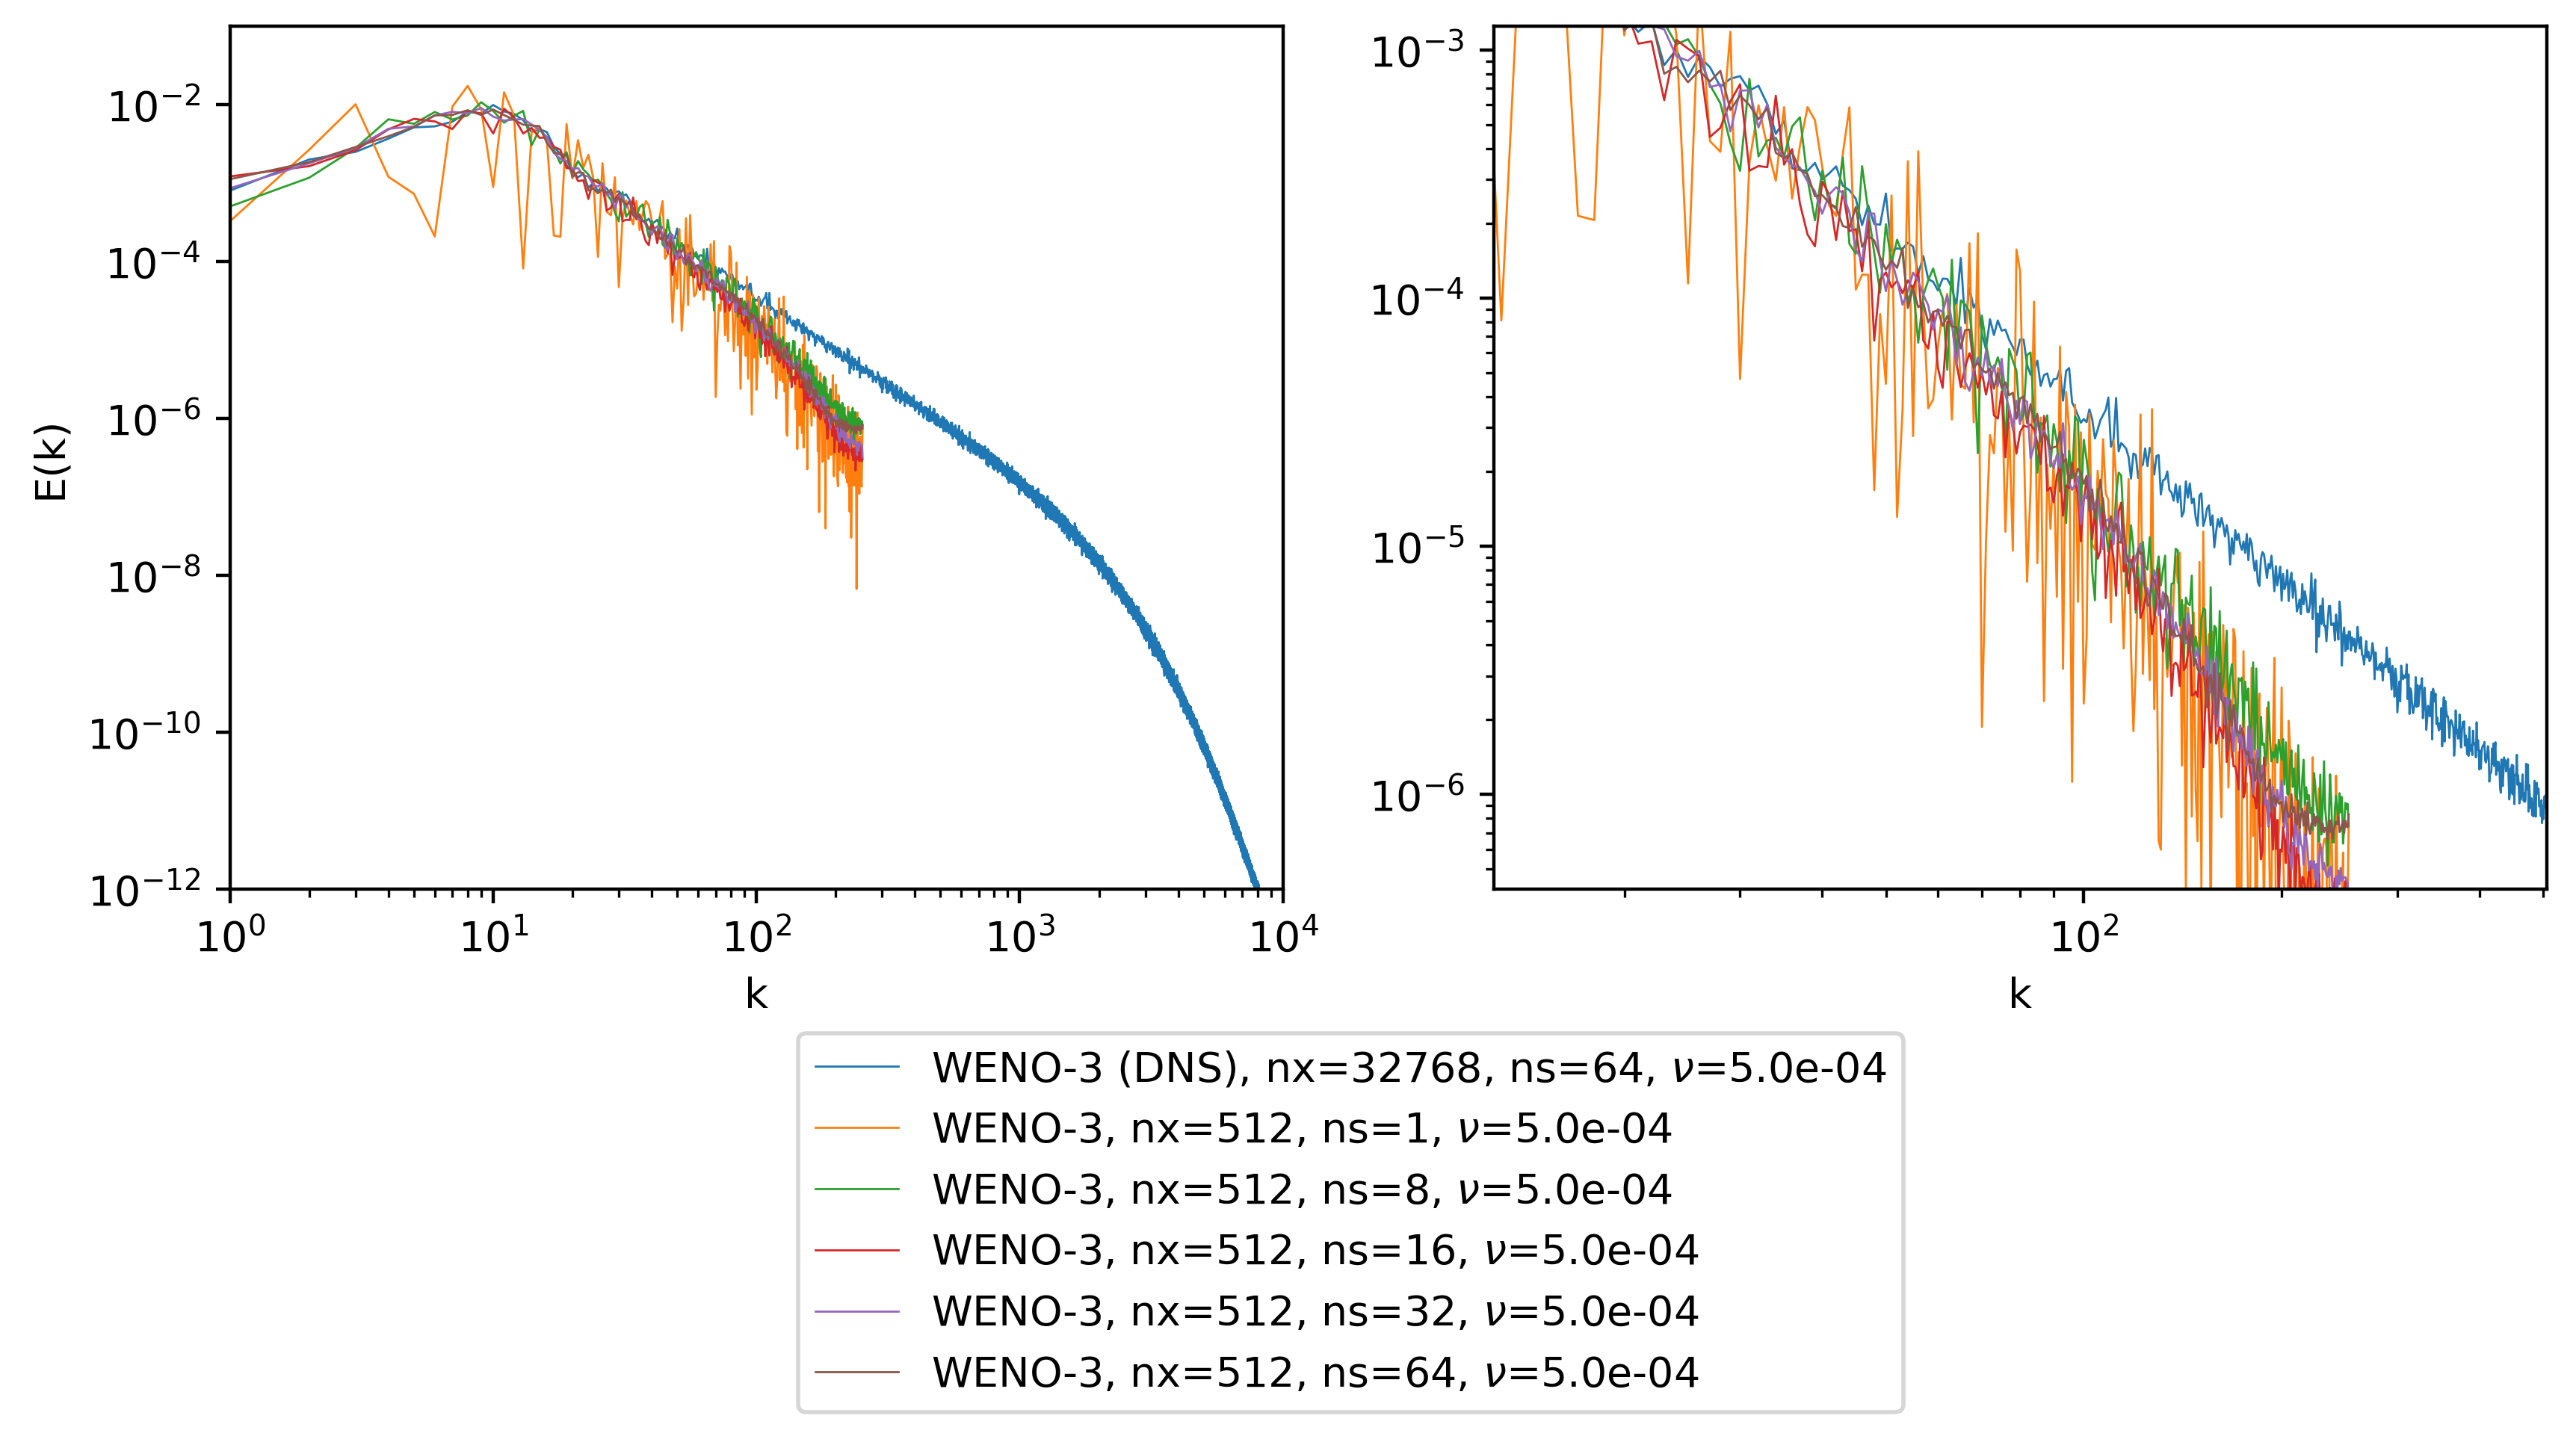
\includegraphics[width=0.75\textwidth]{figures/WENO3_No_Samples_Comparison_Ek_vs_k.png}
	\caption{Comparison of number of samples, ns, used in $\mathbf{3^{rd}}$
	order WENO results, $\mathbf{t=0s}$}
	\label{fig:no_samples}
\end{figure}

Once the initial velocity field is generated in wavenumber space, an FFT is
used to convert to physical space, $u(t)$. This field can then be advanced in
time using the subsequently defined numerical methods. In order to compare
numerical schemes, we will obtain the kinetic energy spectrum in wavenumber
space, $E(k)$, total kinetic energy, $E(t)$, and kinetic energy dissipation
rate, $-dE(t)/dt$, defined by:

\begin{equation}
	E(k) = \frac{1}{2} |\hat{u}(k)|^2 \textit{,} \quad \quad \quad
	E(t) = \int_{-k_m}^{k_m} E(k) dk \textit{,} \quad \quad \quad
	-\frac{dE(t)}{dt} = \frac{E(t) - E(t-\Delta t)}{\Delta t}
\end{equation}


\section{Numerical Methods} \label{sec:numerical}

\subsection{Finite Volume Formulation}

As mentioned in section \ref{sec:gov_eqn}, the finite volume formulation is
well-suited for the Burgers turbulence problem. This is because it is flux
conservative. To show this visually, Figure \ref{fig:finite_volume} shows nodes
$0 \le i \le NX$ at the centers of the finite volume cells. This is where
quantities are stored. Fluxes cross the cell interfaces at nodes $i\pm1/2$. The
primary purpose of this study is to compare various schemes that reconstruct
cell-centered quantities ($i$) at the cell interfaces ($i\pm1/2$). As will be
seen in the results, different schemes have different levels of dissipative
effects on the solution. It should also be noted that it was chosen to use 2
ghost points on the lefthand-side of the domain ($-2, -1$), and 3 ghost points
on the righthand-side of the domain ($NX+1, NX+2, NX+3$). This definition
becomes apparent in the wave speed definition in section \ref{sec:time_int}.

\begin{figure}[hbt!]
	\centering
	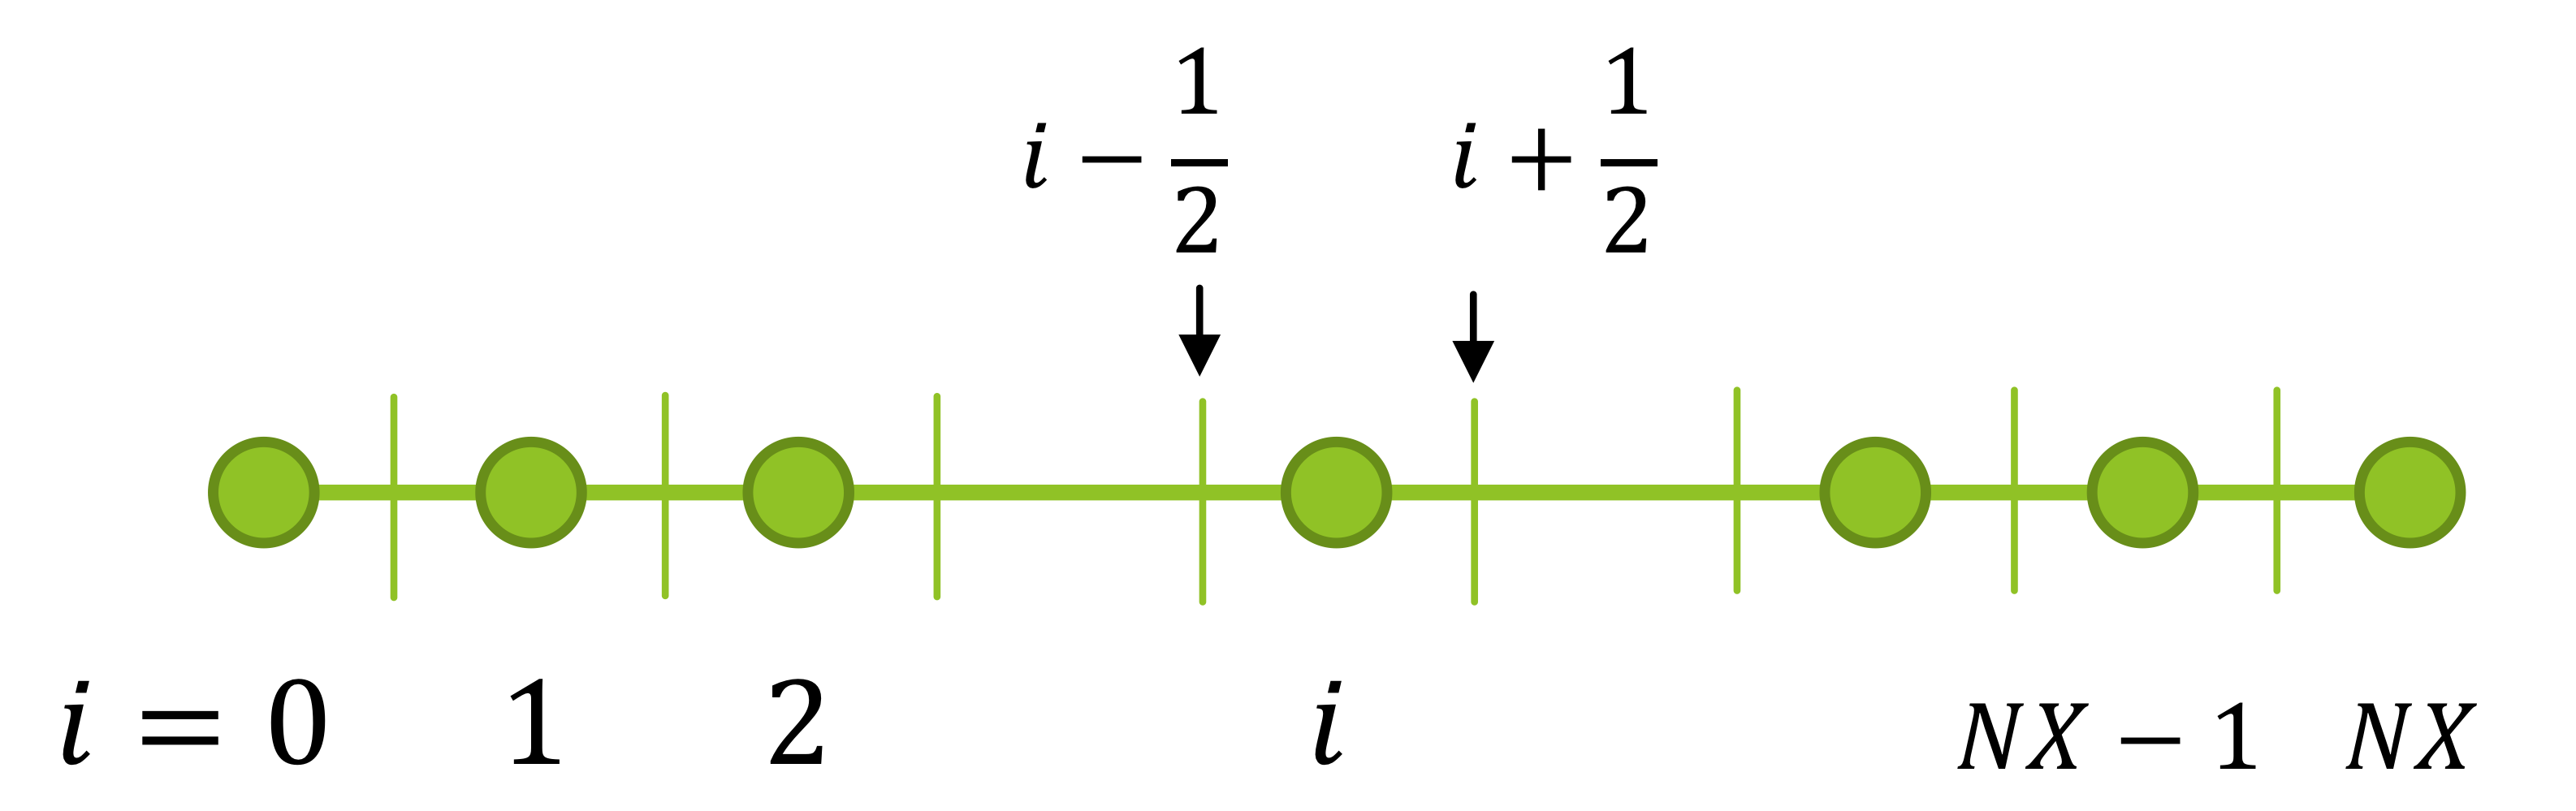
\includegraphics[width=0.5\textwidth]{figures/Finite_Volume.png}
	\caption{Finite Volume Formulation}
	\label{fig:finite_volume}
\end{figure}

\subsection{Algorithm}

To integrate and solve the viscous Burgers equation over time, we will use the
following algorithm, which incorporates techniques like third-order Runge Kutta
for time integration, a 4th order compact scheme for the second
derivative, and various flux-based solvers for the inviscid term:

\begin{itemize}
	\item Outer Loop, Time Integration (with index $n$):
	\begin{enumerate}
		\item Determine $\Delta t$ for stability.
		\item Integrate over time to get $u^n \rightarrow u^{n+1}$:
		\begin{itemize}
			\item Get viscous right-hand side (RHS) of update equation using
				$4^{th}$ order compact scheme.
			\item Get inviscid RHS using Rusanov Riemann solver and one of
				several finite volume reconstruction schemes.
		\end{itemize}
	\end{enumerate}
\end{itemize}

We will first quickly go over the $\Delta t$ determination, Runge-Kutta
integration scheme, and $4^{th}$ order compact scheme, before entering the
focus of the paper: finite volume reconstruction schemes.

\subsection{Time Integration} \label{sec:time_int}
To update $u^n$ in time, we will use a $3^{rd}$ order Runge Kutta algorithm,
which is described by:
\begin{equation}
	\begin{aligned}
		& u^{(1)} = u^n + \Delta t \cdot \mathit{RHS}(u^n) \\
		& u^{(2)} = \frac{3}{4} u^n + \frac{1}{4} u^{(1)} +
		            \frac{1}{4} \Delta t \cdot \mathit{RHS}(u^{(1)}) \\
		& u^n     = \frac{1}{3} u^n + \frac{2}{3} u^{(2)} +
					\frac{2}{3} \Delta t \cdot \mathit{RHS}(u^{(2)})
	\end{aligned}
\end{equation}
where $RHS(u)$ is the right hand side of Eqn. \ref{eq:gov_eqn} when
rearranged for $(\partial u / \partial t)$. After each intermediate $u^{(n)}$
calculation, periodic boundary conditions are enforced to ensure the ghost
points on the left and righthand-sides of the domain are updated accordingly.

To integrate and obtain a stable solution, we must choose a $\Delta t$ that
meets the following stability criterion \cite{maulik2018explicit}:

\begin{equation}
	\Delta t = \textit{CFL}
	\frac{\Delta x}{\text{max} \left(c_{i+1/2}^n \right)}
\end{equation}
where $c_{i+1/2}^n$ are the wave speeds at the cell interfaces, $i+1/2$, given
by:

\begin{equation}
	c_{i+1/2}^n = \text{max} \left( |u_{i-2}|, |u_{i-1}|, |u_i|, |u_{i+1}|,
	                                |u_{i+2}|, |u_{i+3}| \right)
	\text{;} \quad
	0 \le i \le NX
\end{equation}

\subsection{Compact Scheme for Second Derivative}

To obtain the second derivative, $u''$, from the viscous portion of the
governing equation, we will use the following $4^{th}$ order compact scheme:

\begin{equation}
	\frac{1}{10} u''_{i-1} + u''_i + \frac{1}{10} u''_{i+1} =
	\frac{6}{5h^2} \left( u_{i+1} - 2u_i + u_{i-1} \right)
\end{equation}
which can be solved using a cyclic Thomas Algorithm \cite{shanbhag_2014}.

\subsection{Reconstruction Schemes for Solving Inviscid Burgers Equation}
After using the compact scheme to solve for $(\partial^2 u / \partial x^2)$, we
just need to solve for $u (\partial u / \partial x)$ to complete the $RHS$ for
time integration. This can be found using the same techniques that would solve
the inviscid Burgers equation:

\begin{equation}
	\frac{\partial u}{\partial t} = -u \frac{\partial u}{\partial x}
\end{equation}

There are two main methods to do this: reconstruction schemes (which we will be
focusing on) and flux-splitting schemes. The idea is to reconstruct the
cell-centered values, $u_i$, at the cell interfaces, $u_{i+1/2}$, using
primarily nodes from either the left-hand or right-hand sides $\left(
u_{i+1/2}^L \text{ or } u_{i+1/2}^R \text{ respectively} \right)$. From there, we
get the left and right fluxes, $F^{L/R}=F \left(u_{i+1/2}^{L/R} \right)$, and
solve for the flux at the cell interface using the Rusanov Riemann solver:

\begin{equation}
	F_{i+1/2} = \frac{1}{2} \left( F^R + F^L \right) - \frac{c_{i+1/2}}{2}
	\left( q_{i+1/2}^R - q_{i+1/2}^L \right)
\end{equation}
where here, $q=u$.  Once we have $F_{i+1/2}$, the rest is simple:

\begin{equation}
	u \frac{\partial u}{\partial x} = \frac{1}{\Delta x} \left( F_{i+1/2} -
		F_{i-1/2} \right)
\end{equation}
The primary solution differences in this study are the different reconstruction
schemes used to obtain $u_{i+1/2}^{L/R}$. While there are many not included
here, we will focus on the MUSCL and WENO reconstruction schemes.

\subsubsection{MUSCL Reconstruction}
One method for reconstructing quantities at the cell interface is called
Monotone Upwind-Central Schemes for Conservation Laws (MUSCL). This method has
many variants and makes use of flux limiters to prevent new maximums or
minimums from arising in the simulation. A one-parameter MUSCL scheme can be
described by \cite{san2014numerical}:

\begin{equation}
	\begin{aligned}
		q_{i+1/2}^L &= q_i + \frac{1}{4} \left[
			(1-\kappa) \phi \left( \frac{1}{r} \right) (q_i - q_{i-1}) +
			(1+\kappa) \phi(r) (q_{i+1} - q_i)
		\right] \\
		q_{i+1/2}^R &= q_i - \frac{1}{4} \left[
			(1+\kappa) \phi \left( \frac{1}{r} \right) (q_i - q_{i-1}) +
			(1-\kappa) \phi(r) (q_{i+1} - q_i)
		\right] \\
	\end{aligned}
\end{equation}
where $\kappa$ is a parameter that changes the type of MUSCL scheme, $\phi$ is
a limiter function, and
\[
	r = \frac{q_i - q_{i-1}}{q_{i+1} - q_i}
\]

Because the parameter $\kappa$ and limiter function $\phi$ are able to be
changed, a variety of MUSCL scheme variants can be formed using different
values and combinations of values. The different types of MUSCL schemes studied
in this paper are shown in Table \ref{t:muscl_types}, while the various limiter
functions are described in Table \ref{t:limiters}.

\begin{table}[hbt!]
\caption{\label{t:muscl_types} Different types of MUSCL schemes formed by
different choices of $\kappa$ \cite{san2014numerical}.}
\centering
\begin{tabular}{rl|rl}
\hline
      Scheme & $\kappa$ value(s) &          Scheme & $\kappa$ value(s) \\
\hline
	  Quick: &             $0.5$ &             KT: &           $1, -1$ \\
	Central: &               $1$ & $3^{rd}$ Order: &             $1/3$ \\
	 Upwind: &              $-1$ &          Fromm: &               $0$ \\
\hline
\end{tabular}
\end{table}

\begin{table}[hbt!]
\caption{\label{t:limiters} Different limiters and their definitions
         \cite{san2014numerical}}
\centering
\begin{tabular}{c|ll}
\hline
Limiter Type & \multicolumn{2}{c}{Definition} \\
\hline
Van Leer & $\phi_{vl}(r) = \frac{r + |r|}{1+r}$ &
           $\lim\limits_{r \to \infty} \phi_{vl}(r) = 2$ \\
Van Albada & $\phi_{va}(r) = \frac{r^2 + r}{r^2 + 1}$ &
		     $\lim\limits_{r \to \infty} \phi_{va}(r) = 1$ \\
Min-Mod & $\phi_{mm}(r) = \max \left( 0, \min(r, 1) \right)$ &
           $\lim\limits_{r \to \infty} \phi_{mm}(r) = 1$ \\
Superbee & $\phi_{sb}(r) = \max \left( 0, \min(2r, 1), \min(r, 2) \right)$ &
           $\lim\limits_{r \to \infty} \phi_{sb}(r) = 2$ \\
Monotonized Central & $\phi_{mc}(r) = \max \left( 0, \min(2r, 0.5(1+r), 2) \right)$ &
                      $\lim\limits_{r\to\infty} \phi_{mc}(r) = 2$  \\
\hline
\end{tabular}
\end{table}

\subsubsection{WENO Reconstruction: \texorpdfstring{$3^{rd}$}{3rd} Order}
Another method for reconstructing quantities at the cell interface is called
the Weighted Essentially Non-Oscillatory (WENO) scheme. This makes use of
smoothness indicators, $\beta_k$, which indicate the smoothness of the field on
the left and right sides of node $i$. These are then used in conjunction with
linear weights to construct nonlinear weights, $w_k$, which are used to
determine which nodes will have the most impact on the reconstructed cell
interface quantities. If there were a shock discontinuity on the left of node
$i$, for example, the influence of those nodes would be weighted very small.

For the $3^{rd}$ order WENO scheme, the smoothness indicators are definied by:

\begin{equation}
	\beta_1 = \left( q_i - q_{i-1} \right)^2 \textit{;} \quad
	\beta_2 = \left( q_{i+1} - q_i \right)^2
\end{equation}
The linear weights are defined by:

\begin{equation}
	d_1^L = \frac{1}{3} \textit{,} \quad
	d_2^L = \frac{2}{3} \textit{,} \quad
	d_1^R = \frac{2}{3} \textit{,} \quad
	d_2^R = \frac{1}{3}
\end{equation}
The nonlinear weights are defined by:

\begin{equation}
	\alpha_1 = \frac{d_1}{(\beta_1 + \epsilon)^2} \textit{,} \quad
	\alpha_2 = \frac{d_2}{(\beta_2 + \epsilon)^2} \textit{,} \quad
	w_1 = \frac{\alpha_1}{\alpha_1 + \alpha_2} \textit{,} \quad
	w_2 = \frac{\alpha_2}{\alpha_1 + \alpha_2}
\end{equation}
Finally, the $3^{rd}$ order WENO reconstruction at the cell interfaces is given
by:

\begin{equation}
	\begin{aligned}
		q_{i+1/2}^L &= \frac{w_1}{2}(-q_{i-1} + 3q_i) + \frac{w_2}{2}(q_i + q_{i+1}) \\
		q_{i-1/2}^R &= \frac{w_1}{2}(q_{i-1} + q_i) + \frac{w_2}{2}(3q_i - q_{i+1})
	\end{aligned}
\end{equation}

\subsubsection{WENO Reconstruction: \texorpdfstring{$5^{th}$}{5th} Order}

For the $5^{th}$ order WENO scheme, more nodes are required to reconstruct with
increased accuracy. Whereas the $3^{rd}$ order scheme requires nodes from $i-1$
to $i+1$, the $5^{th}$ order scheme requires nodes from $i-2$ to $i+2$. Here, the
smoothness indicators are definied by:

\begin{equation}
\begin{aligned}
\beta_1 &= \frac{13}{12} (q_{i-2} - 2q_{i-1} + q_i)^2 + \frac{1}{4} (q_{i-2} - 4q_{i-1} + 3q_i)^2 \\
\beta_2 &= \frac{13}{12} (q_{i-1} - 2q_i + q_{i+1})^2 + \frac{1}{4} (q_{i-1} - q_{i+1})^2 \\
\beta_3 &= \frac{13}{12} (q_i - 2q_{i+1} + q_{i+2})^2 + \frac{1}{4} (3q_i - 4q_{i+1} + q_{i+2})^2
\end{aligned}
\end{equation}
The linear weights are defined by:

\begin{equation}
	d_1 = \frac{1}{10} \textit{,} \quad
	d_2 = \frac{6}{10} \textit{,} \quad
	d_2 = \frac{3}{10}
\end{equation}
The nonlinear weights are defined by:

\begin{equation}
	\alpha_k = \frac{d_k}{(\beta_k + \epsilon)^2} \textit{,} \quad
	w_k = \frac{\alpha_k}{\sum_k \alpha_k}
\end{equation}
Finally, the $5^{th}$ order WENO reconstruction at the cell interfaces is given
by:

\begin{equation}
\begin{aligned}
	q_{i+1/2}^L &= \frac{w_1}{6}(2q_{i-2} - 7q_{i-1} + 11q_i) +
	               \frac{w_2}{6}(-q_{i-1} + 5q_i + 2q_{i+1}) +
				   \frac{w_3}{6}(2q_i + 5q_{i+1} - q_{i+2}) \\
	q_{i-1/2}^R &= \frac{w_1}{6}(2q_{i+2} - 7q_{i+1} + 11q_i) +
	               \frac{w_2}{6}(-q_{i+1} + 5q_i + 2q_{i-1}) +
				   \frac{w_3}{6}(2q_i + 5q_{i-1} - q_{i-2})
\end{aligned}
\end{equation}


\section{Results}

\subsection{MUSCL Variants \& Limiters Comparison}
When comparing different reconstruction schemes, it is useful to compare how
much dissipation occurs after a certain period of time, in this case $0.05s$.
As shown in Figure \ref{fig:muscl_cs_lim}, some schemes shown higher levels of
kinetic energy than others near the edge of the domain in wavenumber space. The
more kinetic energy, the less dissipative the scheme is. For this study, a high
resolution $3^{rd}$ order WENO (WENO-3) solution was used as the "DNS" result
to compare against. This is considered to be an accurate solution. Figure
\ref{fig:muscl_cs_lim} shows all MUSCL-Central solutions with a limiter show
some amount of dissipation, but the solution without a limiter actually has
more kinetic energy than the DNS solution. This is because the absense of a
limiter allows the numerical scheme to create new maximums and minimums,
introducing error by \textit{adding} kinetic energy. In this case, it is seen
that the Monotonized Central limiter solution is closet to DNS, but in general,
the Superbee limiter showed the best results (see Figure
\ref{fig:muscl_q_lim}).

\begin{figure}[hbt!]
	\centering
	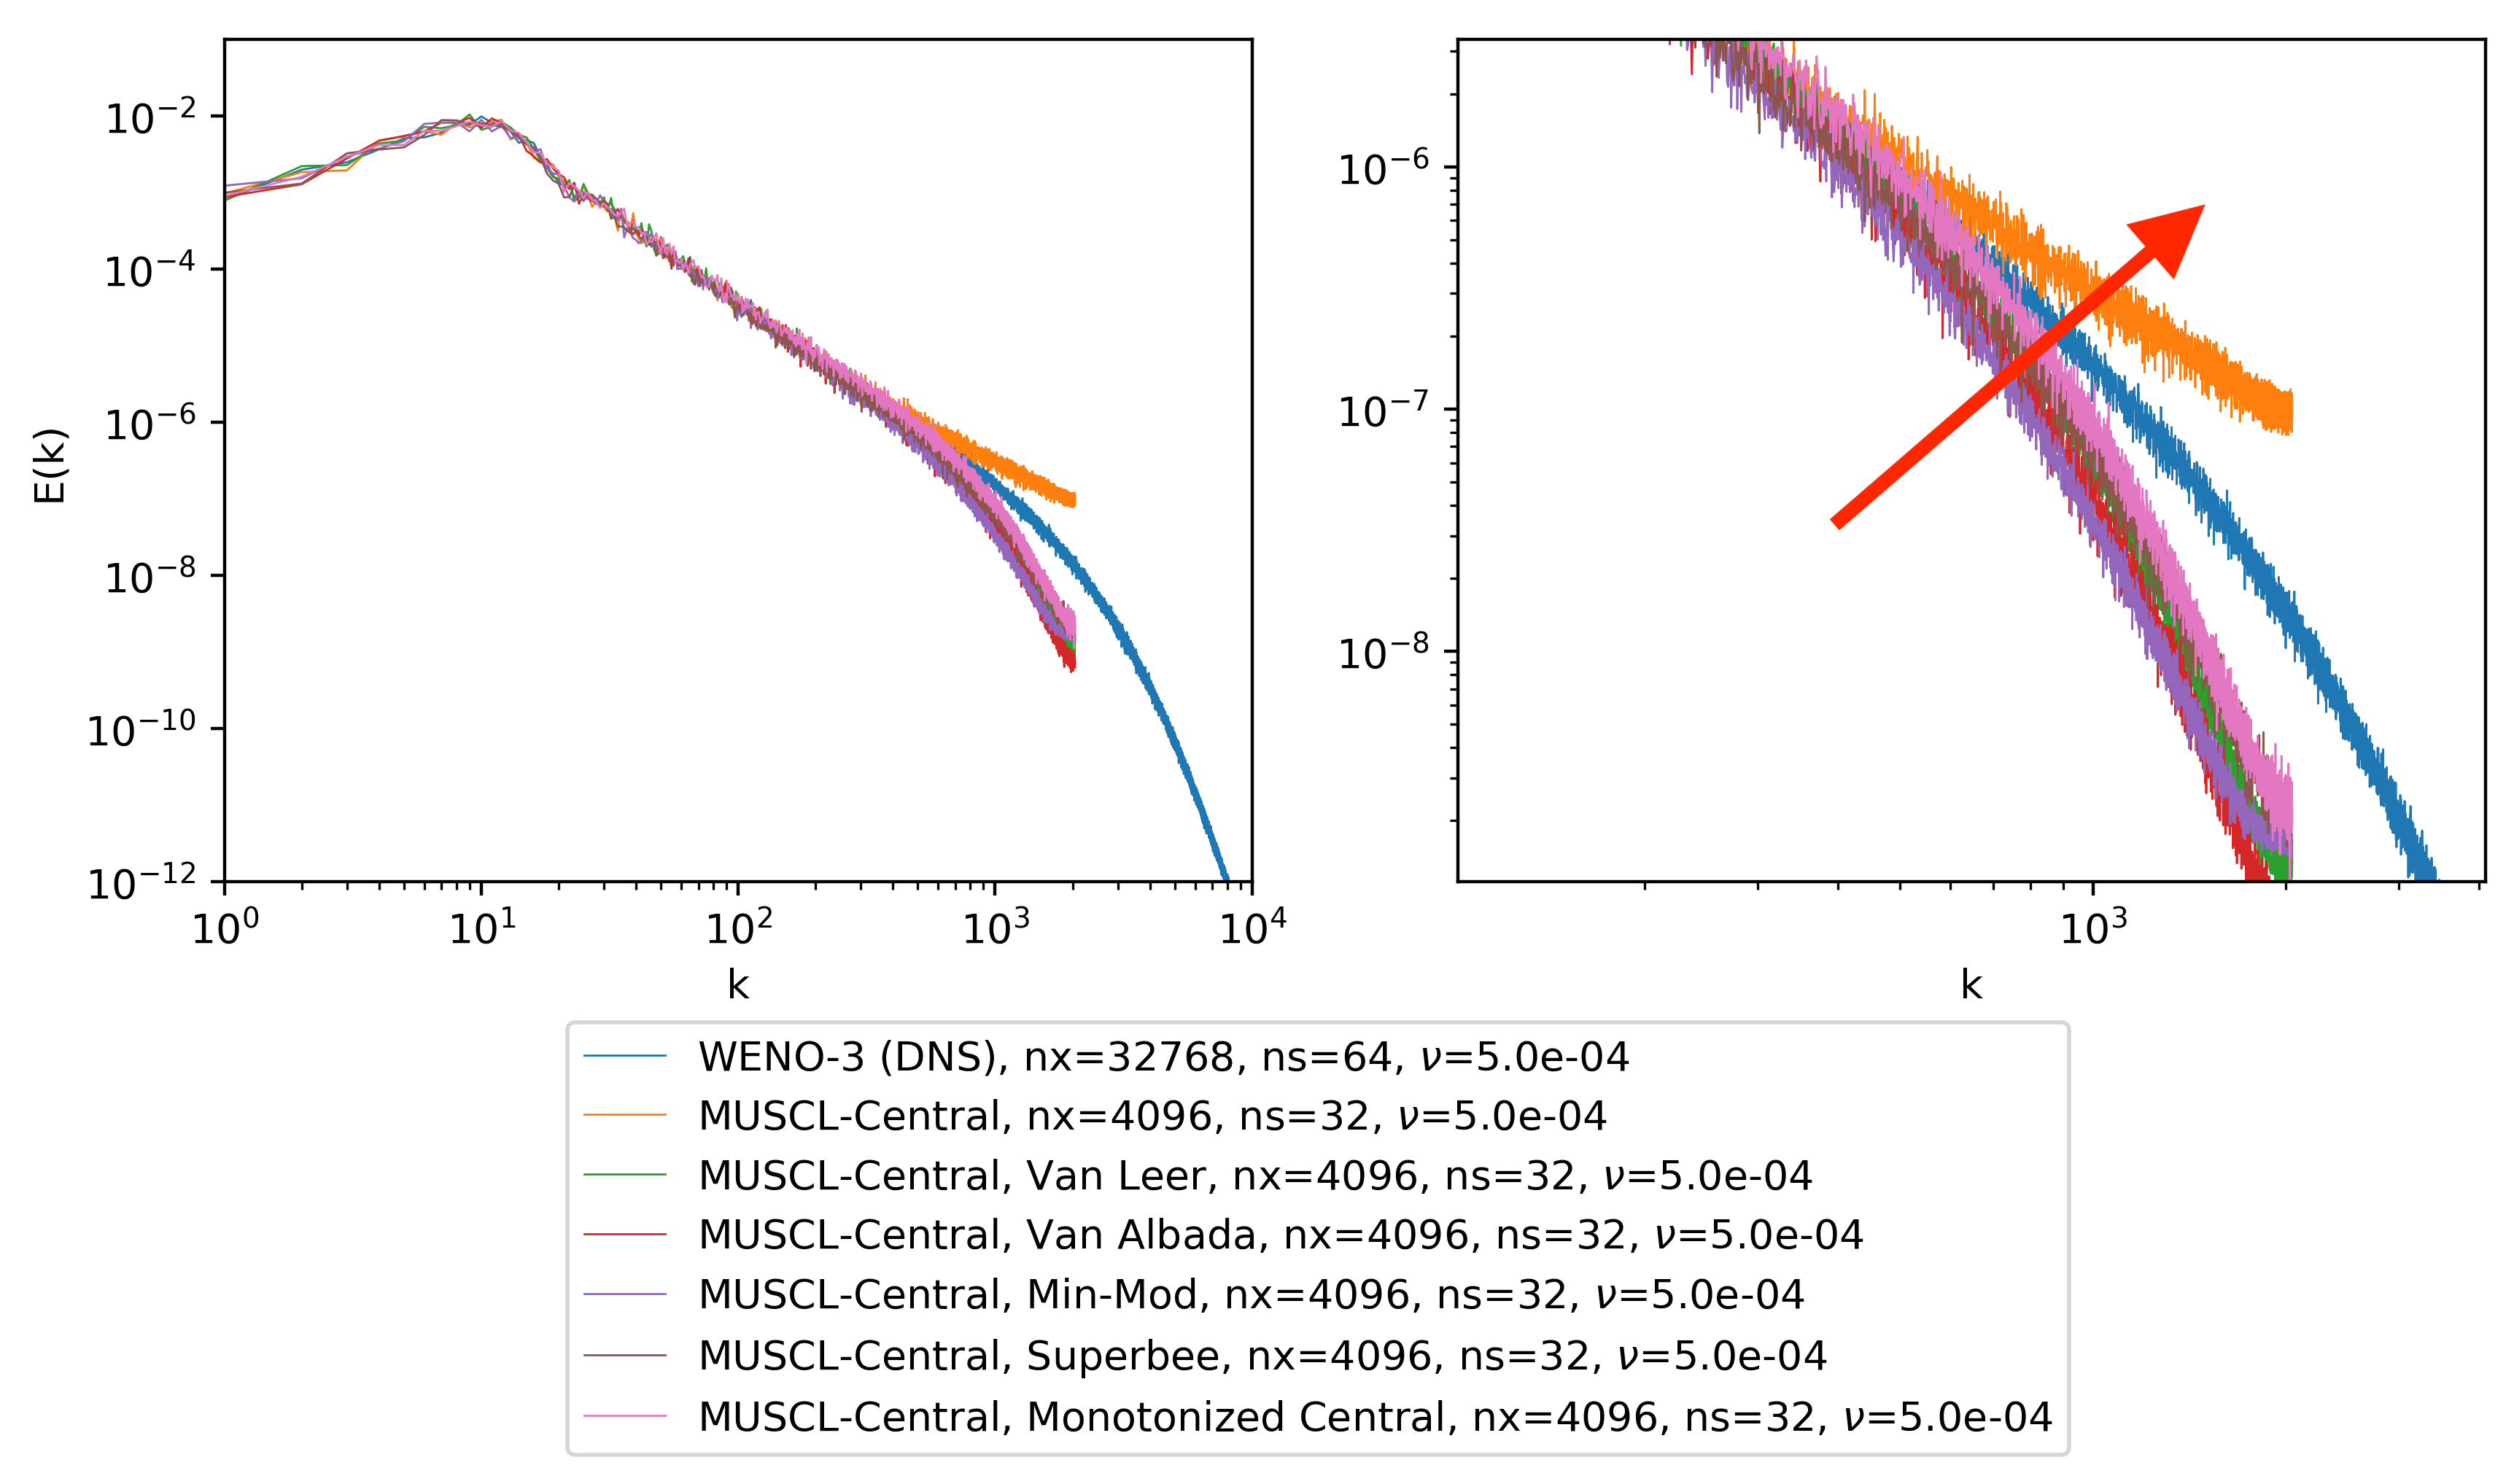
\includegraphics[width=0.75\textwidth]{figures/MUSCL_CS_Limiter_Comparison_Ek_vs_k.png}
	\caption{MUSCL-Central limiter comparison at $t=0.05s$. The red arrow
	indicates that less dissipation occurs as solutions trend towards that
	direction. This is considered to be a desirable characteristic.}
	\label{fig:muscl_cs_lim}
\end{figure}

\begin{figure}[hbt!]
	\centering
	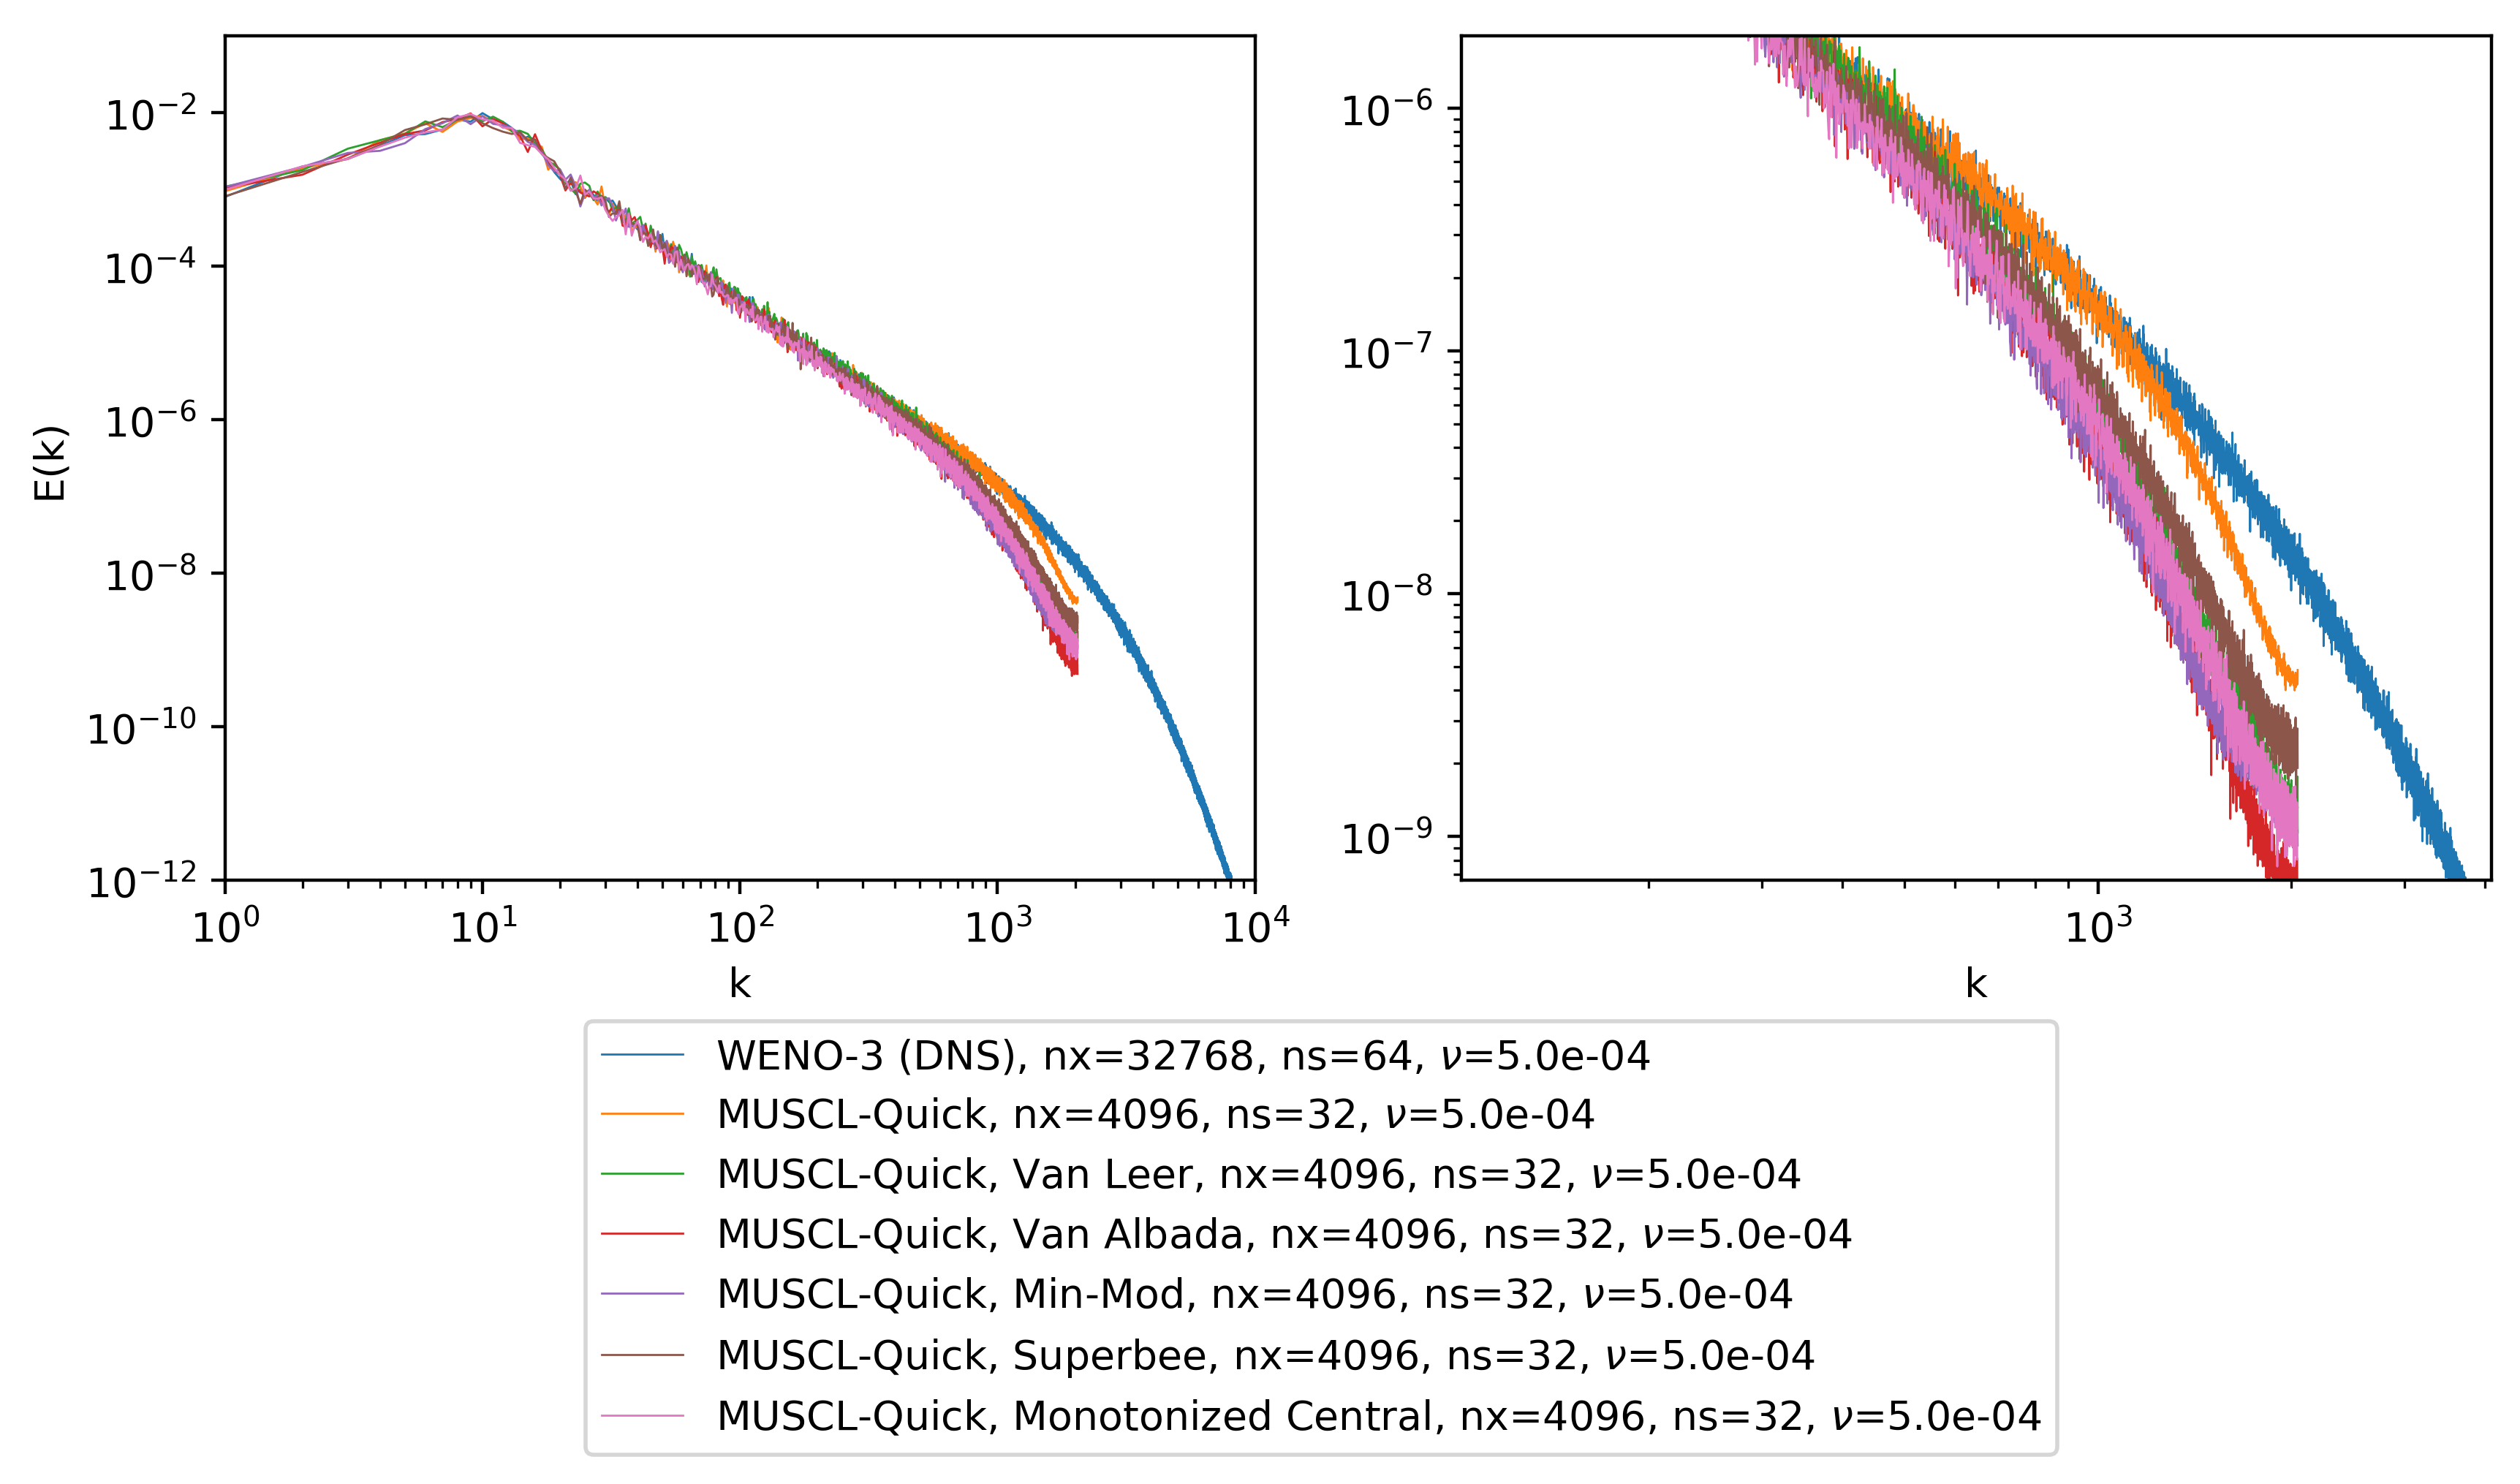
\includegraphics[width=0.75\textwidth]{figures/MUSCL_Q_Limiters_Comparison_Ek_vs_k.png}
	\caption{MUSCL-Quick limiters comparison at $t=0.05s$}
	\label{fig:muscl_q_lim}
\end{figure}

Because Superbee showed the best performance of all the limiters, this was then
used to compare all of the different MUSCL types. The results, shown in Figure
\ref{fig:muscl_sb_type}, show that the type of MUSCL scheme has little impact
on the results when this limiter is applied. More variation is shown between
types, however, when no limiter is applied, as seen in Figure
\ref{fig:muscl_type}. Here it is shown that MUSCL-KT without a limiter
correlates best with the DNS results. This will be used as the best MUSCL
scheme to compare against WENO schemes in section \ref{sec:muscl_vs_weno}.

\begin{figure}[hbt!]
	\centering
	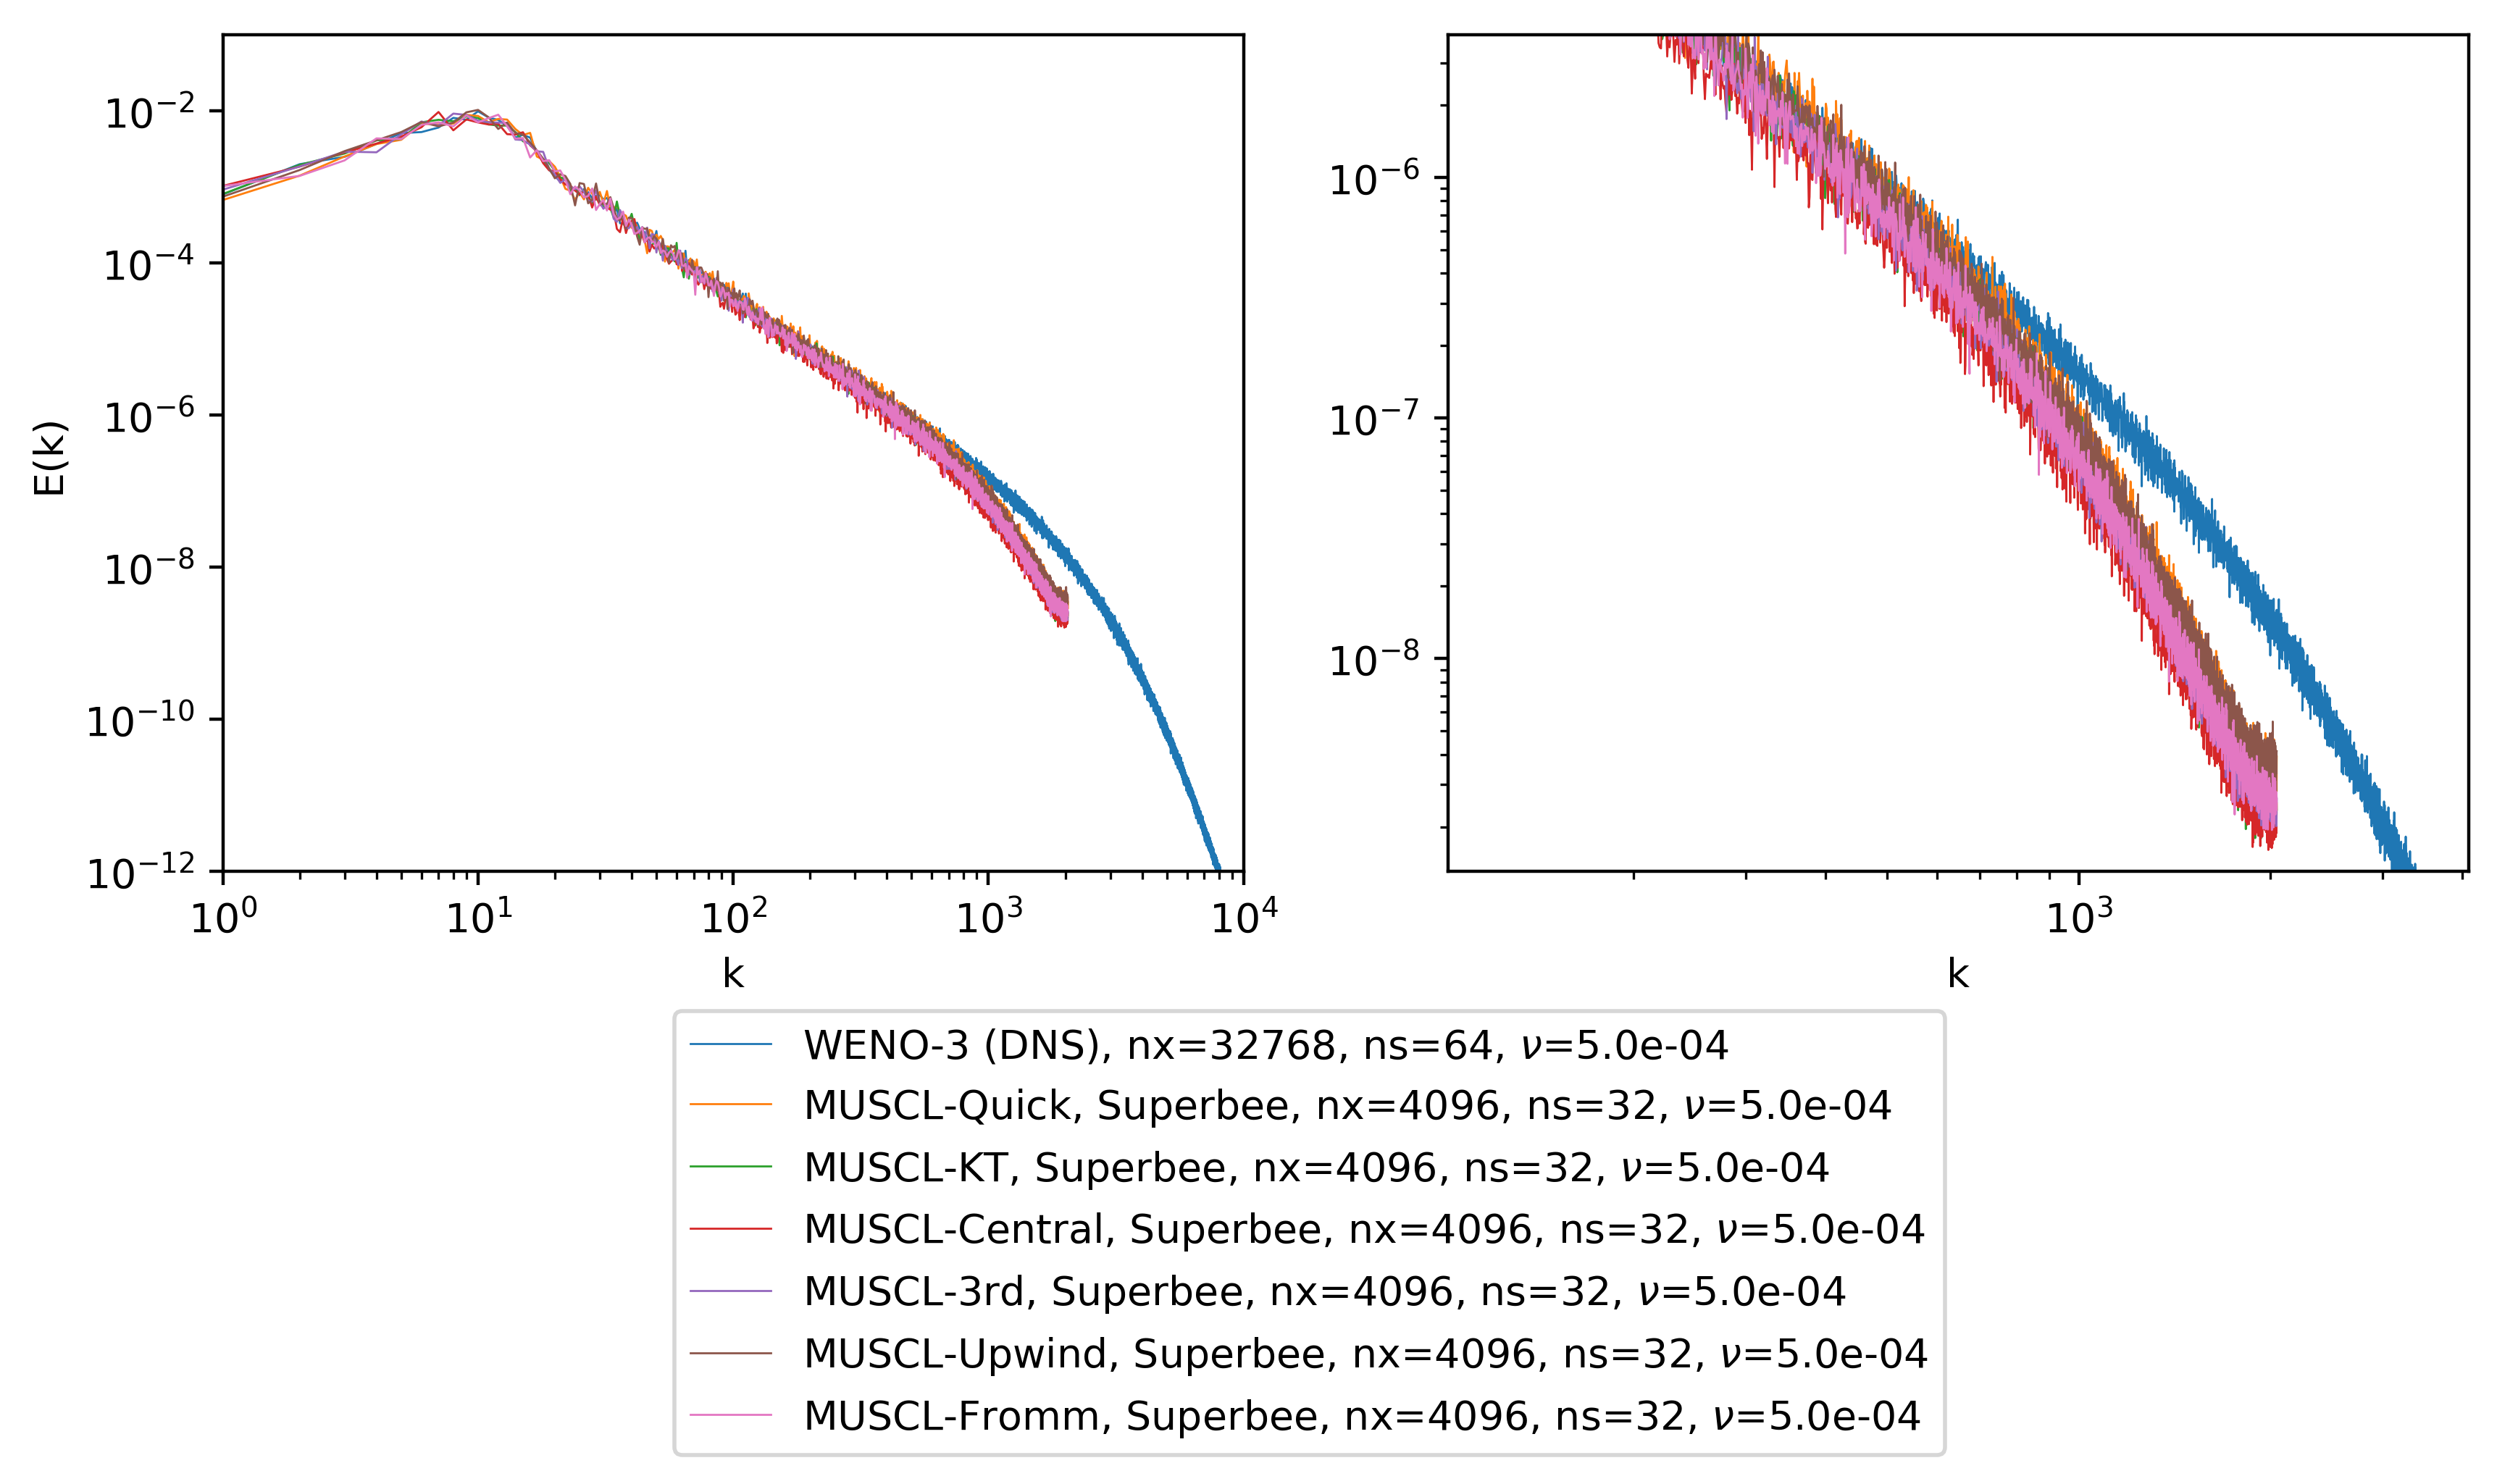
\includegraphics[width=0.75\textwidth]{figures/MUSCL_Superbee_Type_Comparison_Ek_vs_k.png}
	\caption{MUSCL type comparison with Superbee limiter, $t=0.05s$}
	\label{fig:muscl_sb_type}
\end{figure}

\begin{figure}[hbt!]
	\centering
	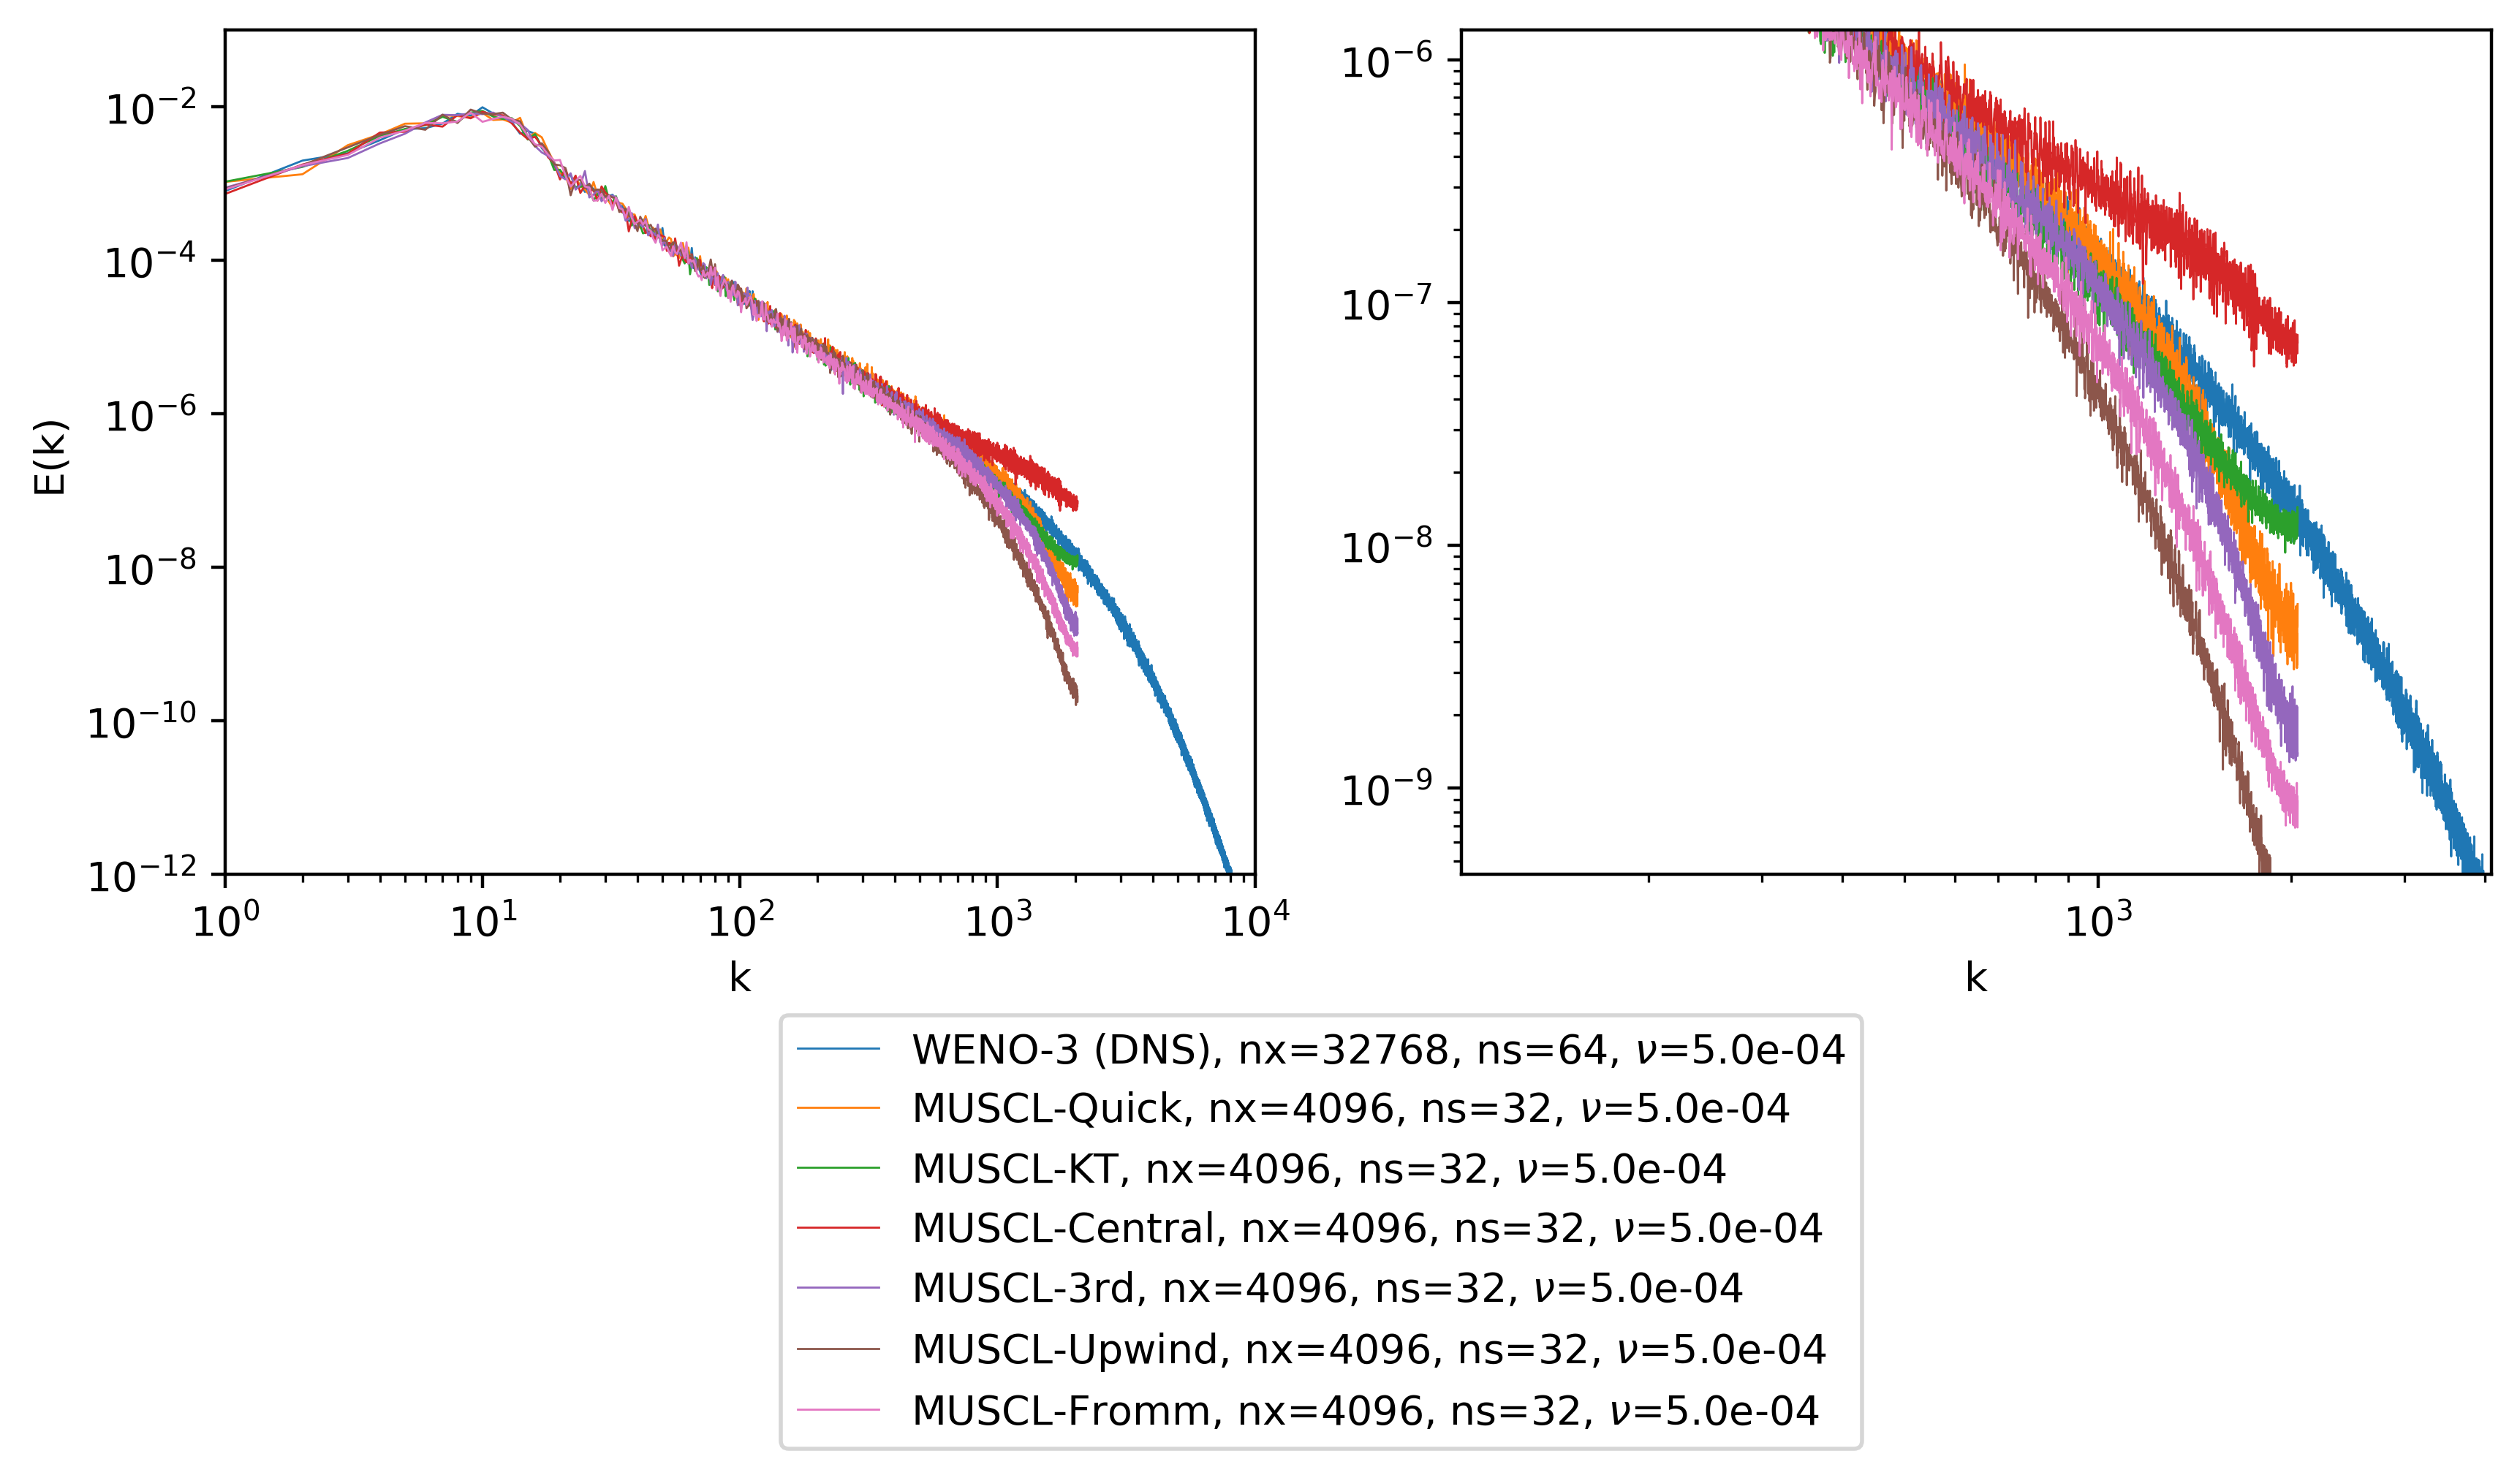
\includegraphics[width=0.75\textwidth]{figures/MUSCL_Type_Comparison_Ek_vs_k.png}
	\caption{MUSCL type comparison without using a limiter, $t=0.05s$}
	\label{fig:muscl_type}
\end{figure}

\subsection{WENO Resolution, Viscosity, and Order Comparisons}

As discussed previously, the solution is considered less dissipative the closer
it is to the DNS results. To show the effect that increasing resolution has on
kinetic energy dissipation, Figure \ref{fig:weno3_res} was produced. This
shows, as expected, that higher resolution solutions produce more accurate and
less dissipative results. Additionally, it was investigated what effect
viscosity had on dissipation, as seen in Figure \ref{fig:weno3_vis}. As
expected, higher viscosity resulted in higher levels of dissipation.

\begin{figure}[hbt!]
	\centering
	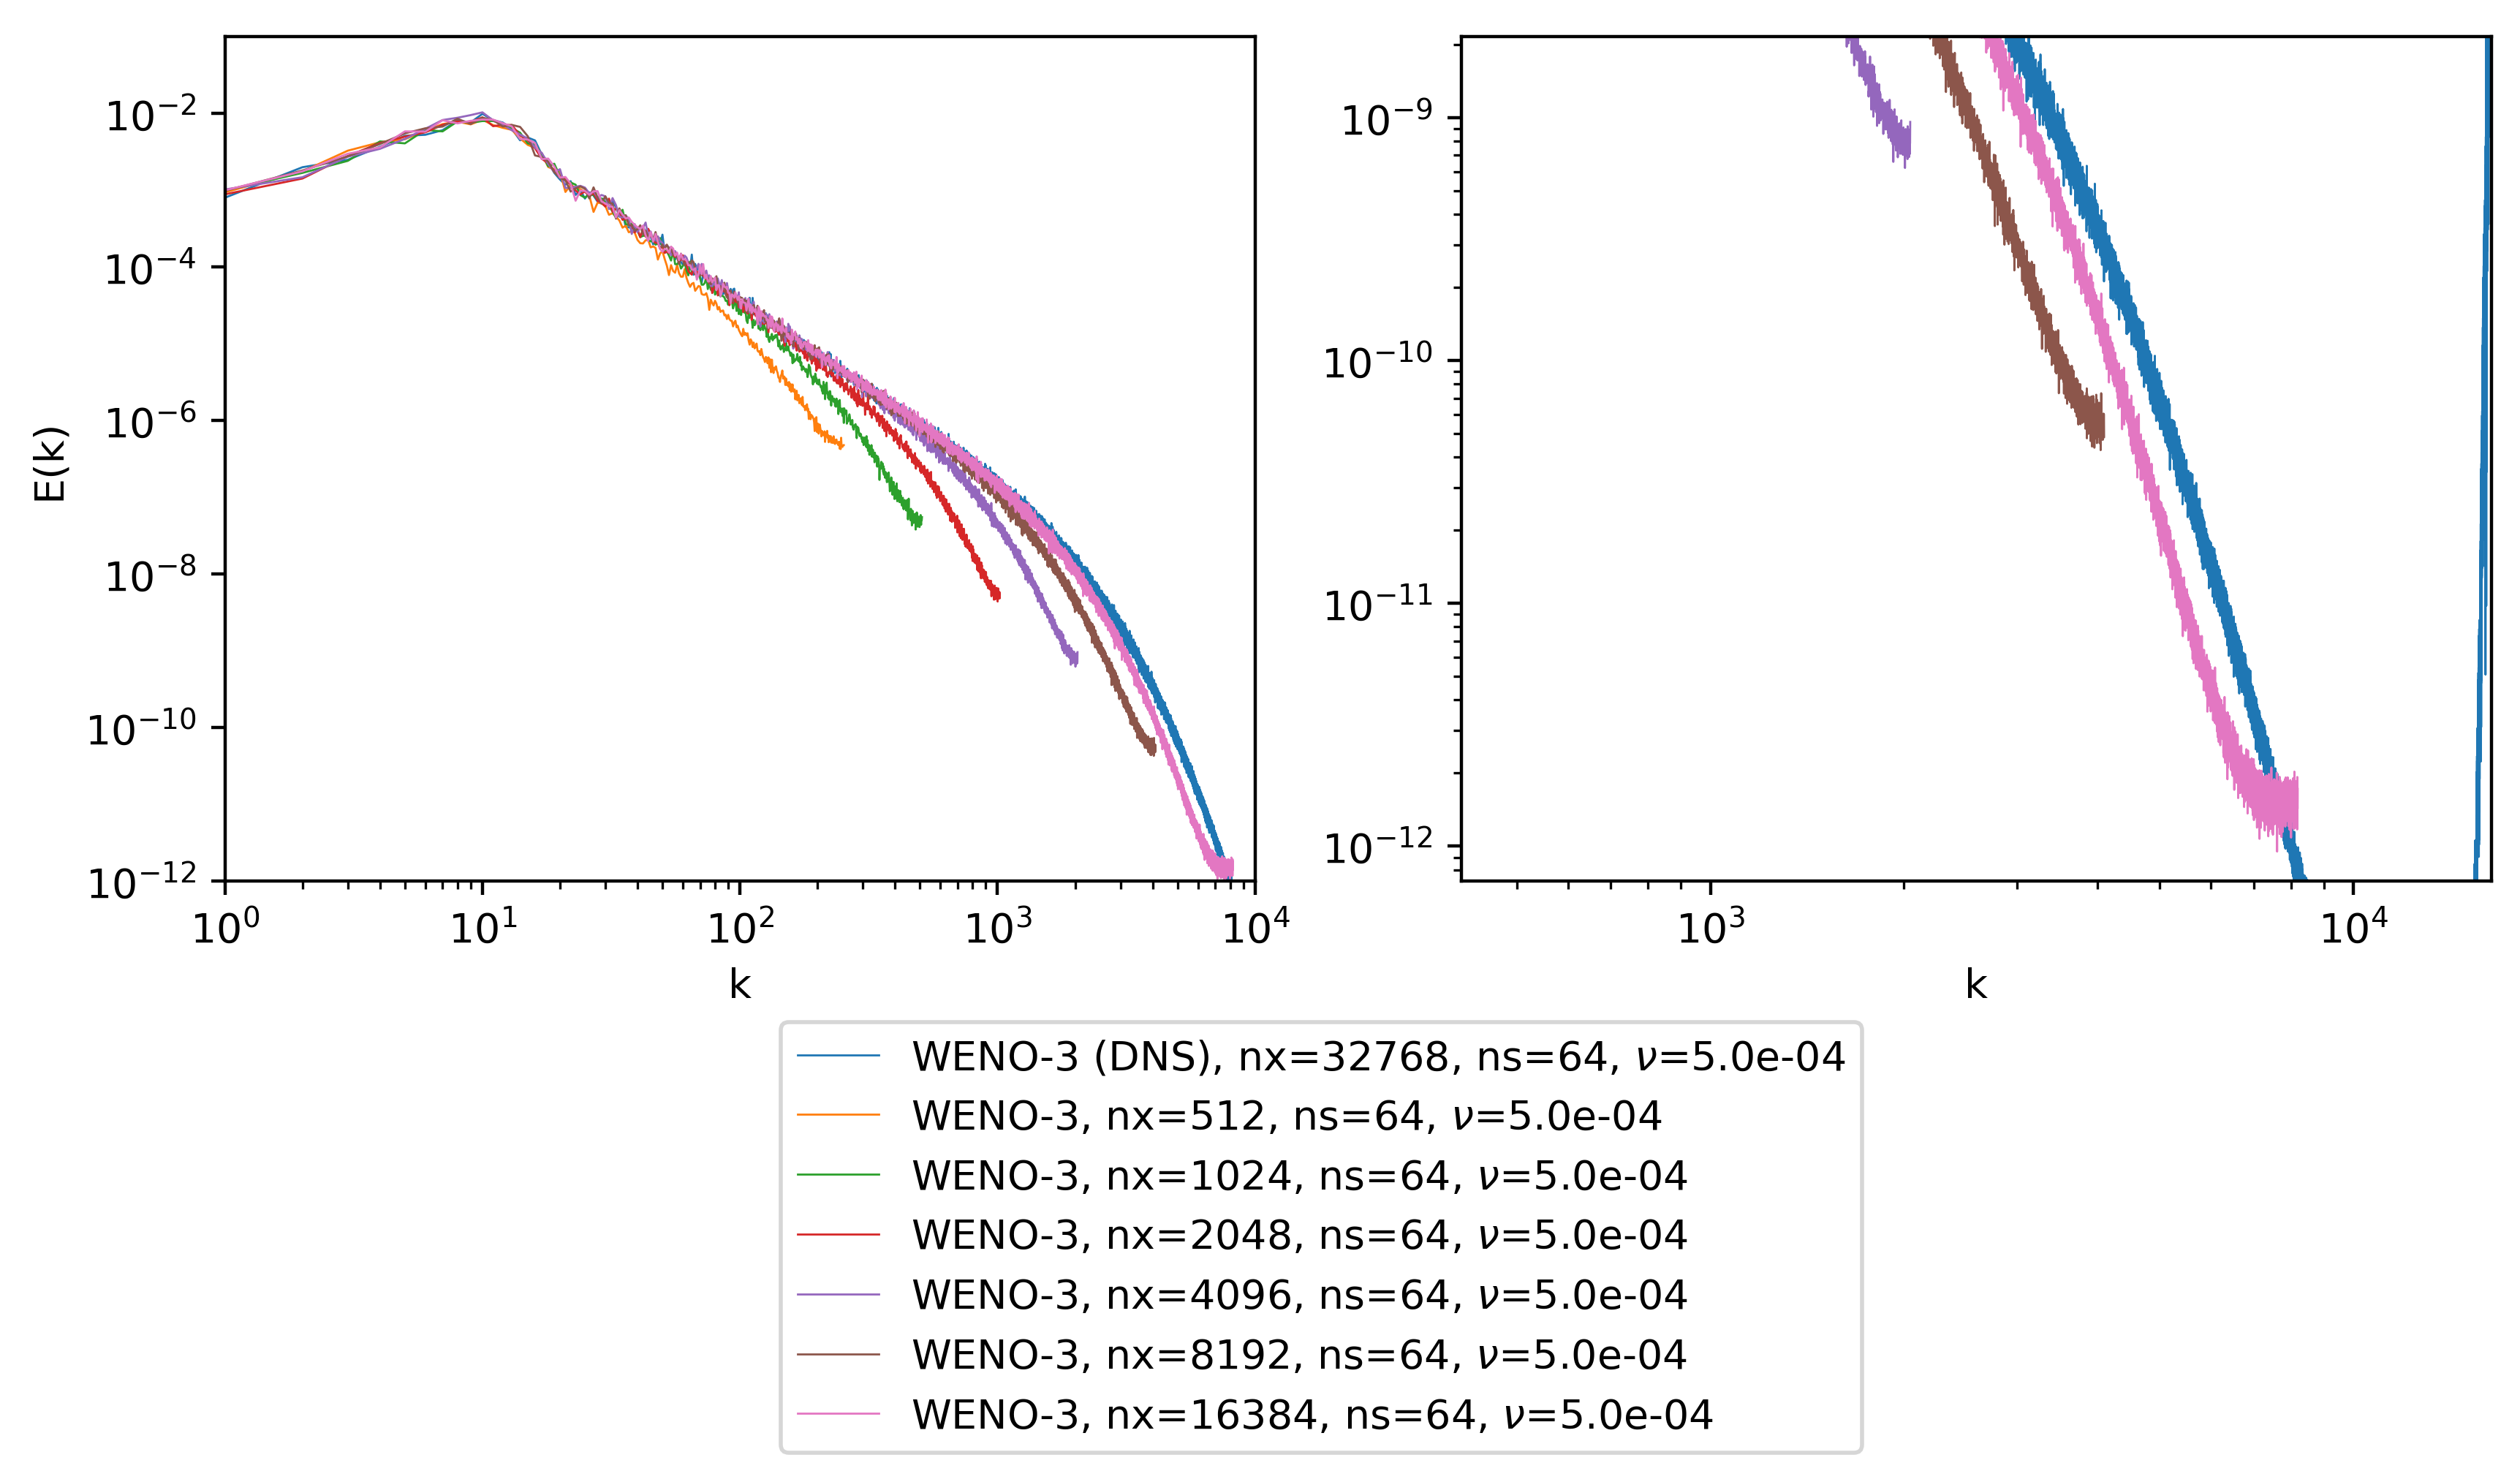
\includegraphics[width=0.75\textwidth]{figures/WENO3_Resolution_Comparison_Ek_vs_k.png}
	\caption{WENO-3 resolution comparison at $t=0.05s$}
	\label{fig:weno3_res}
\end{figure}

\begin{figure}[hbt!]
	\centering
	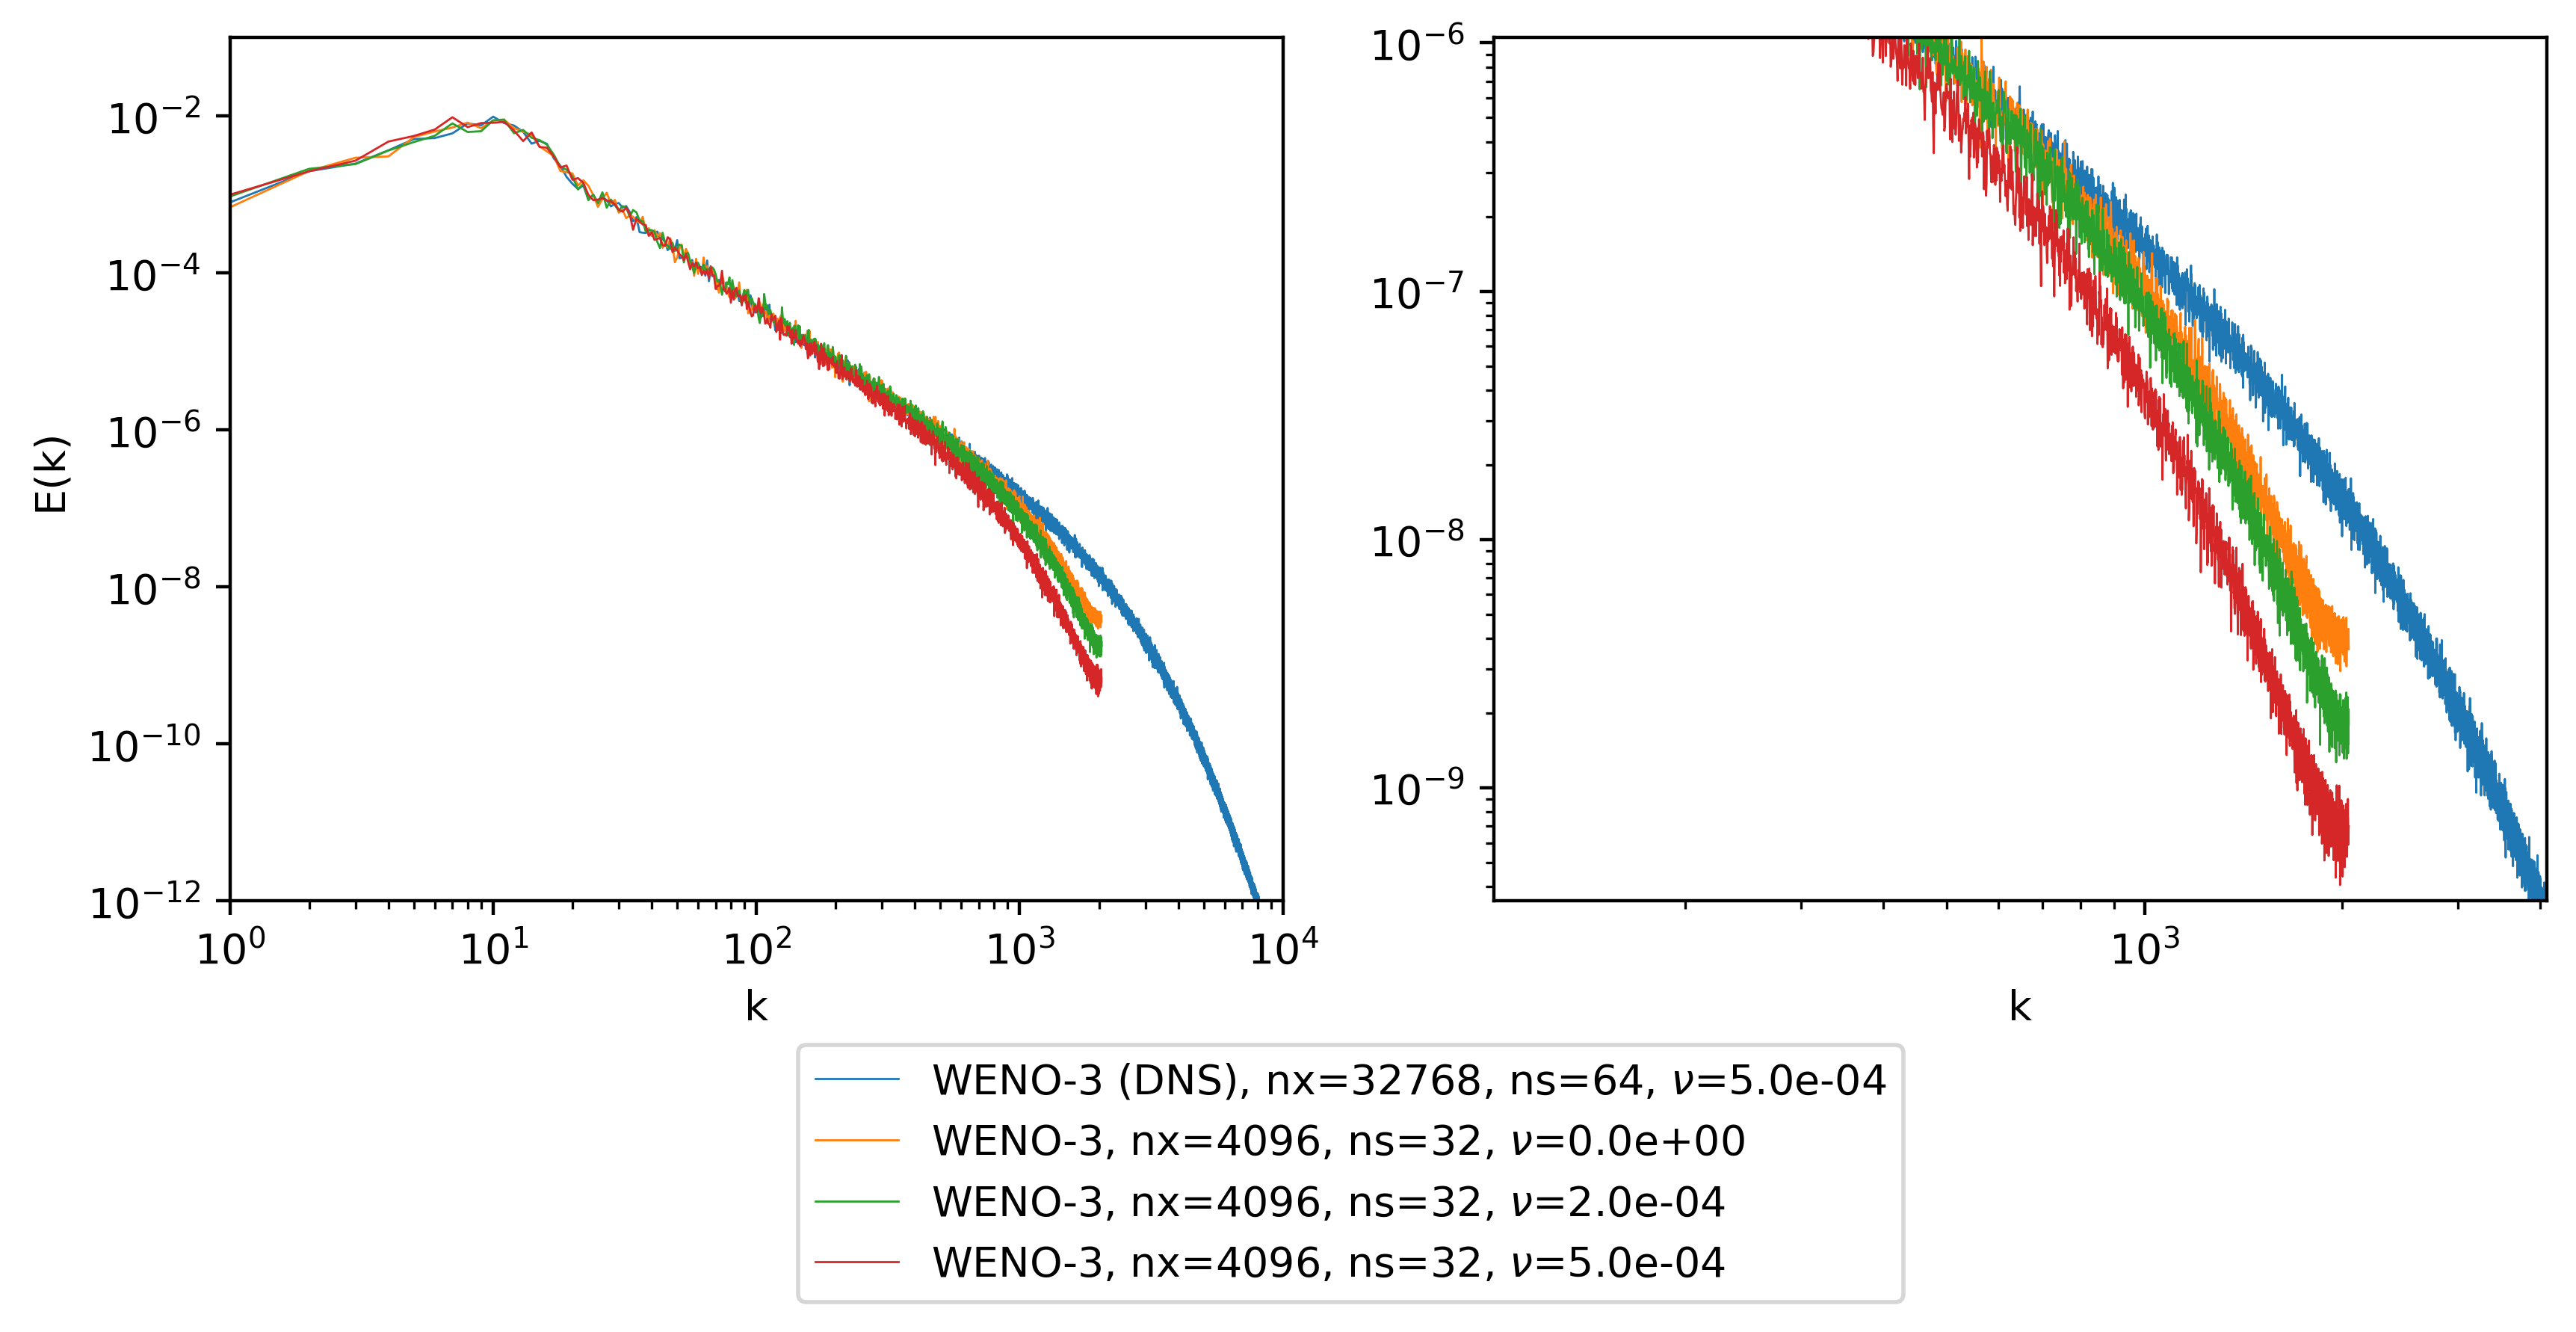
\includegraphics[width=0.7\textwidth]{figures/WENO3_Viscosity_Comparison_Ek_vs_k.png}
	\caption{WENO-3 viscosity comparison at $t=0.05s$}
	\label{fig:weno3_vis}
\end{figure}

The same type of analysis was carried out with the $5^{th}$ order WENO scheme
(WENO-5), and the results are shown in Figures \ref{fig:weno5_res} and
\ref{fig:weno5_vis} respectively. As can be see, all levels of resolution track
fairly well with the WENO-3 DNS result except near the edge of the domain,
where the solution shows dispersive characteristics. More information on this
is discussed in section \ref{sec:dns_type}. As shown by the viscosity comparison in
Figure \ref{fig:weno5_vis}, more viscosity leads to more dissipation, as
expected.

\begin{figure}[hbt!]
	\centering
	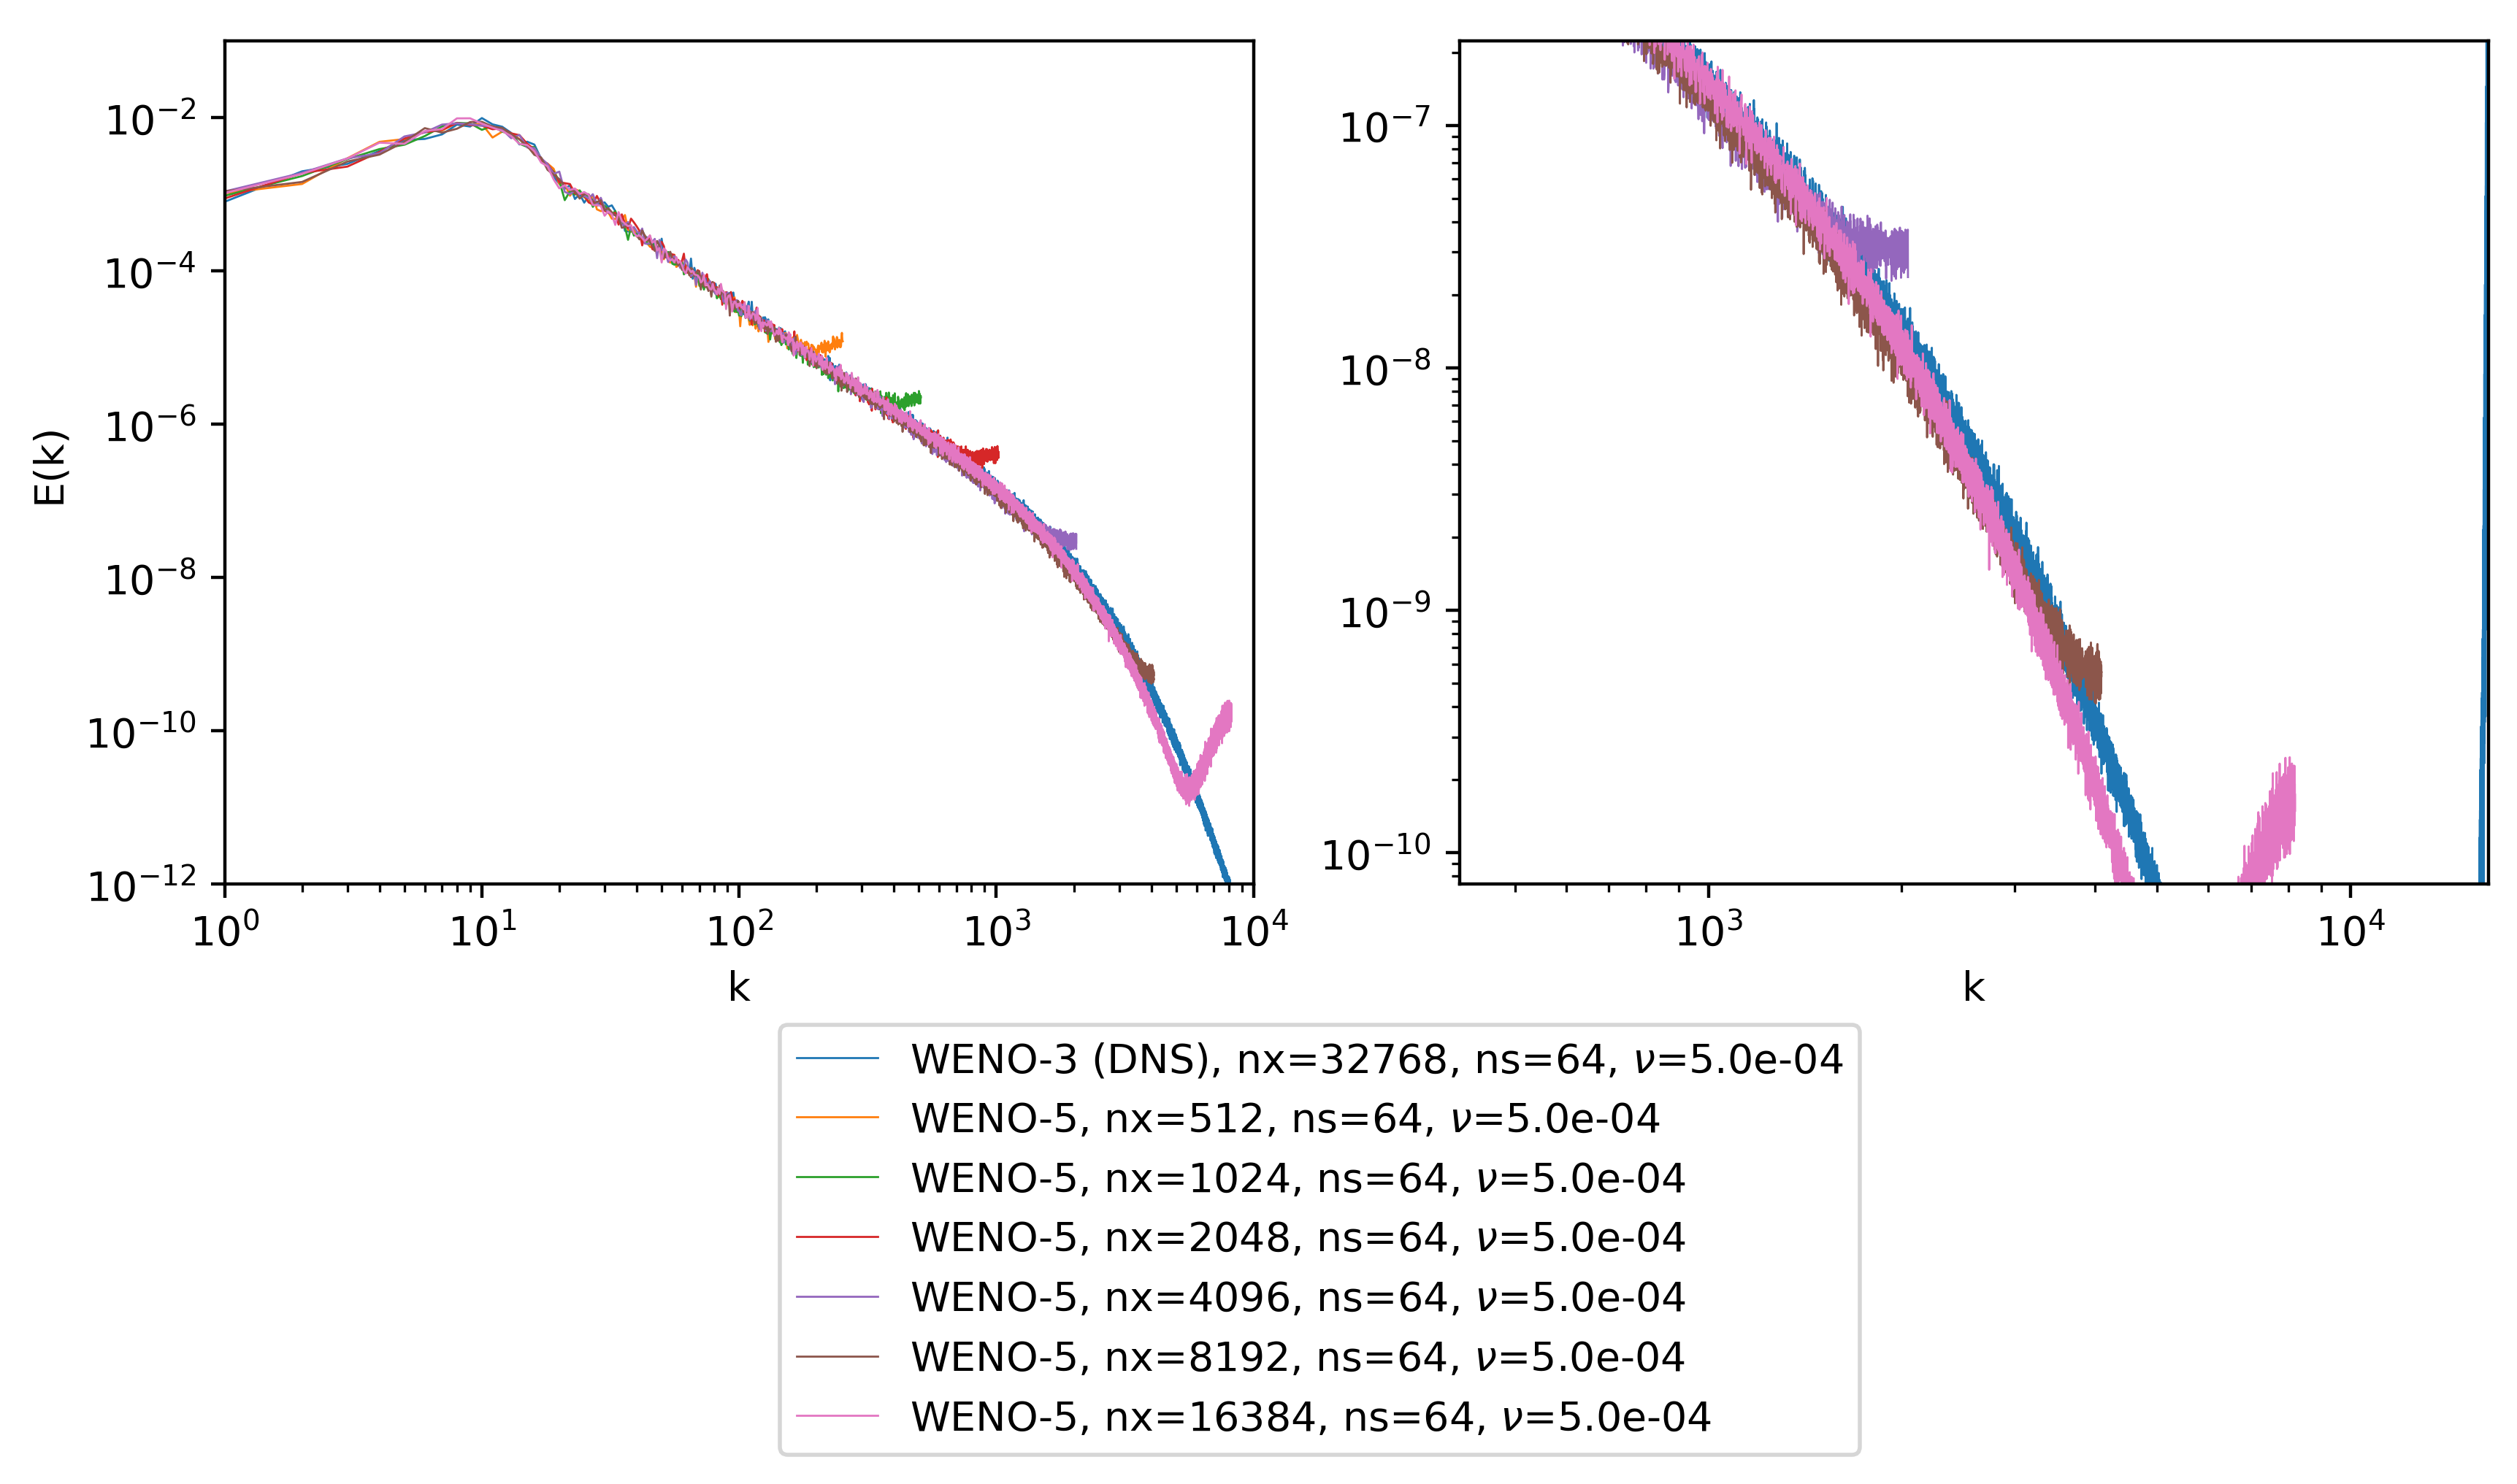
\includegraphics[width=0.7\textwidth]{figures/WENO5_Resolution_Comparison_Ek_vs_k.png}
	\caption{WENO-5 resolution comparison at $t=0.05s$}
	\label{fig:weno5_res}
\end{figure}

\begin{figure}[hbt!]
	\centering
	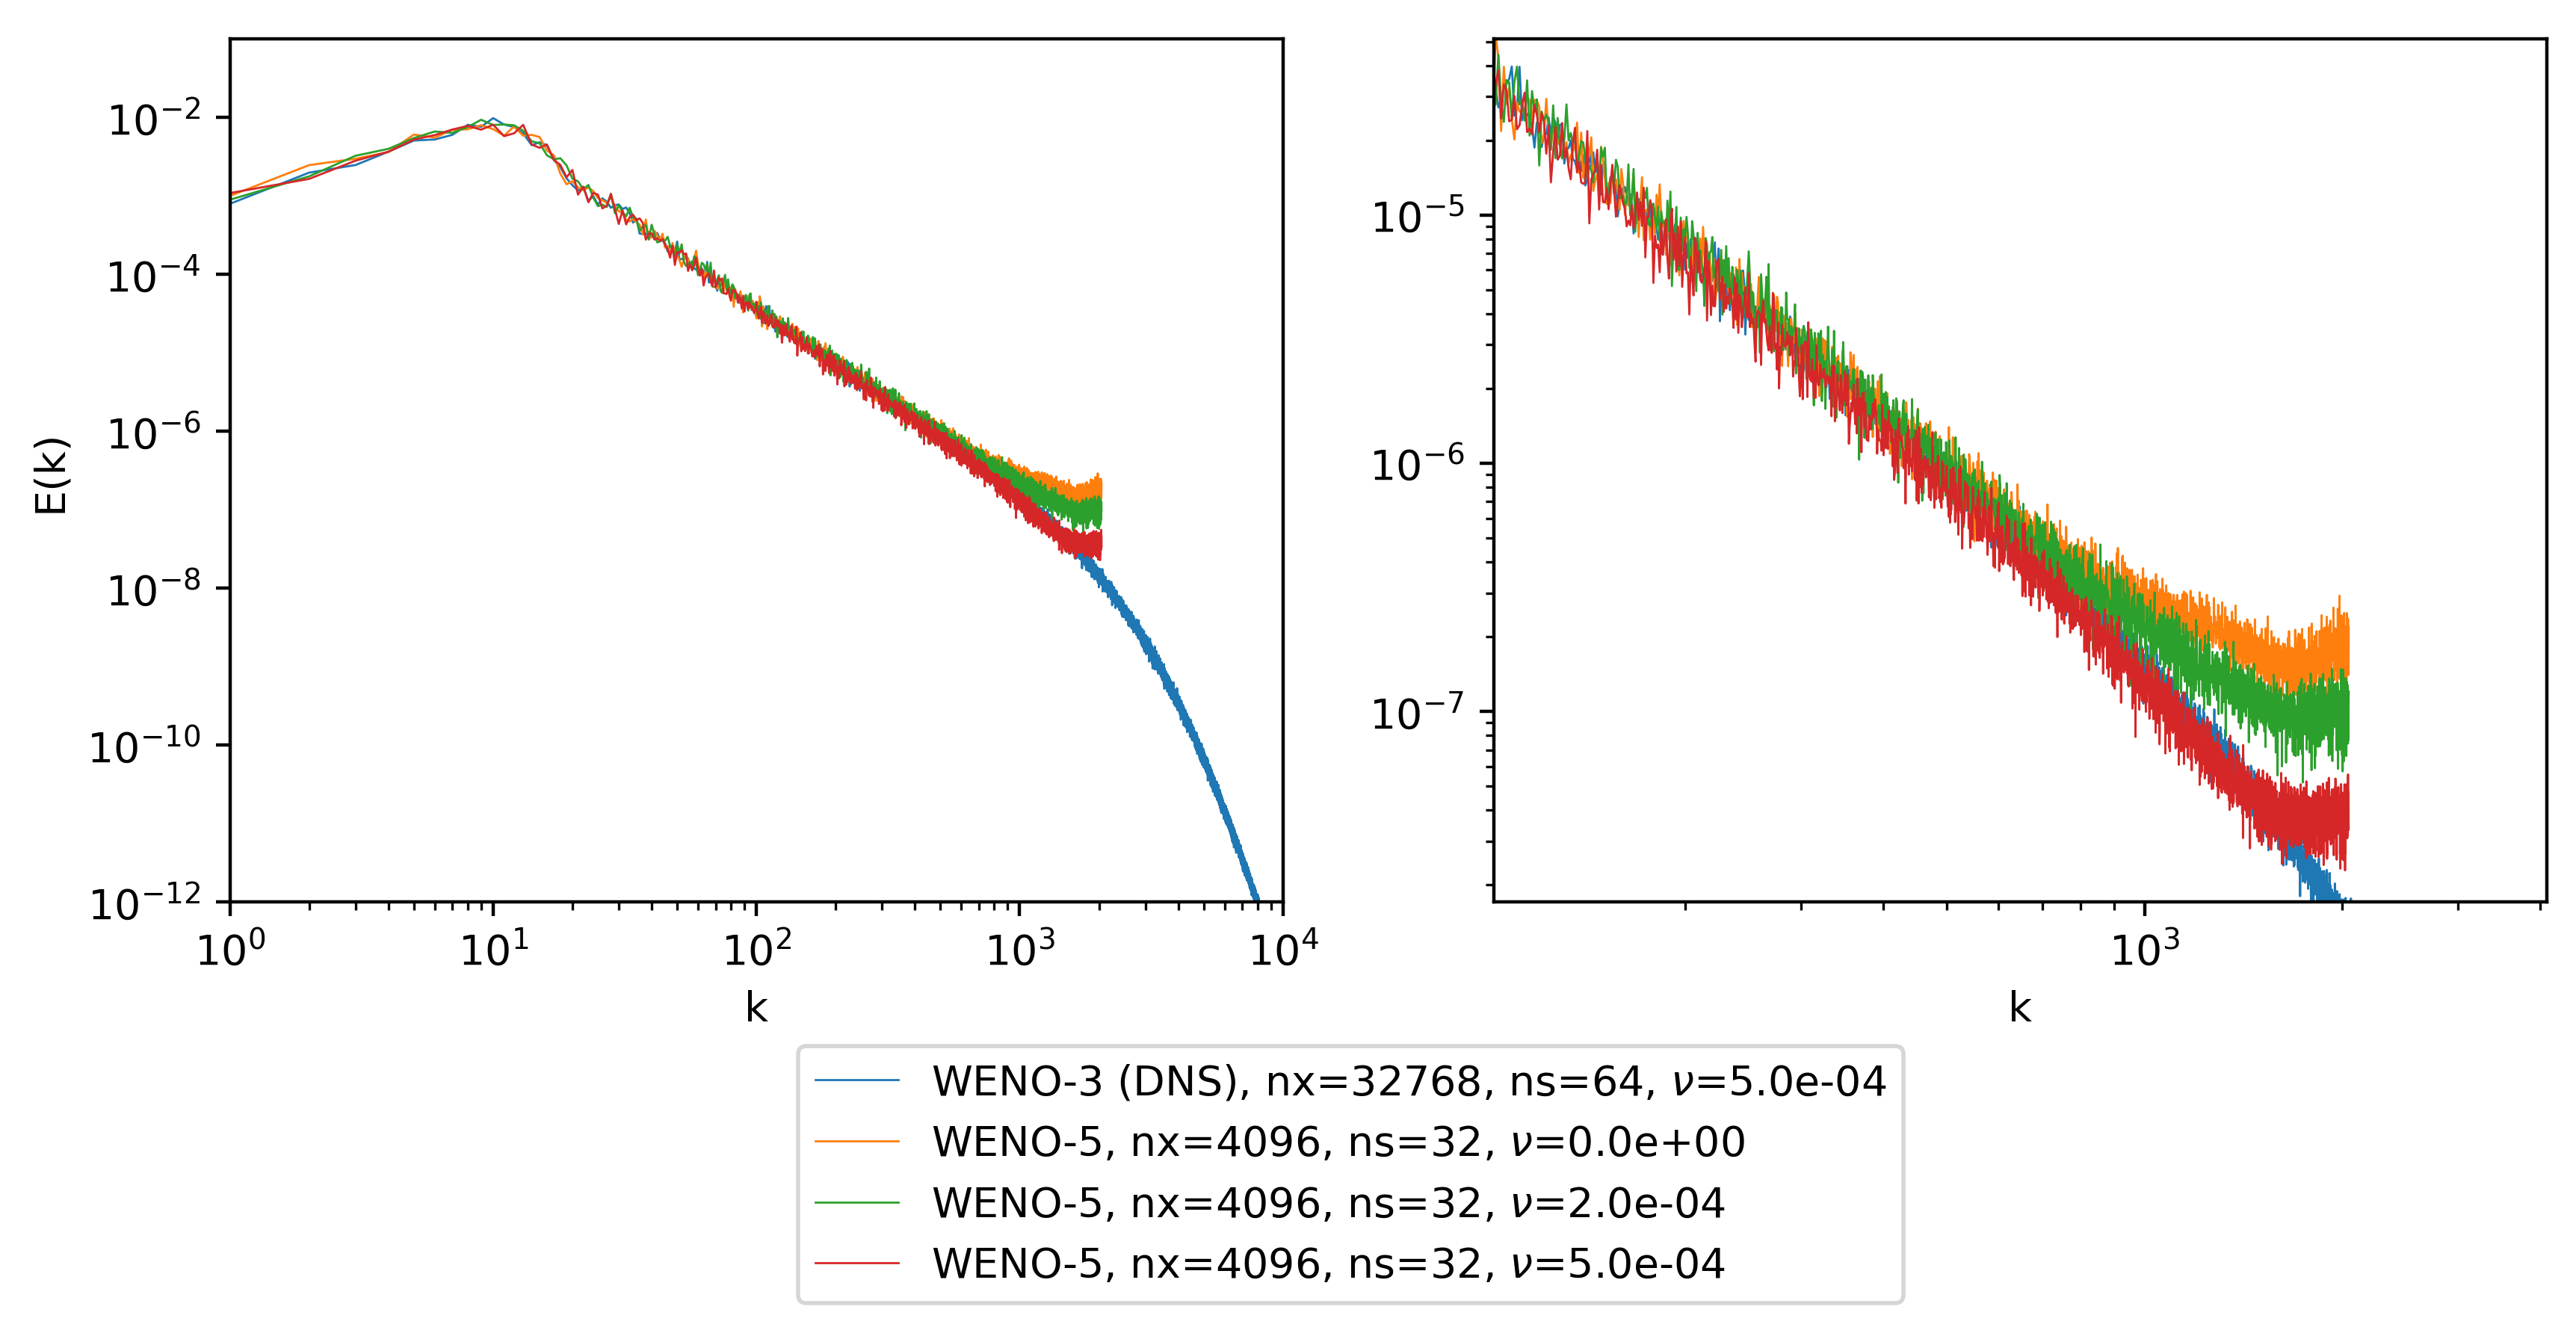
\includegraphics[width=0.7\textwidth]{figures/WENO5_Viscosity_Comparison_Ek_vs_k.png}
	\caption{WENO-5 viscosity comparison at $t=0.05s$}
	\label{fig:weno5_vis}
\end{figure}

When comparing WENO-3 with WENO-5 at the same resolution, WENO-5 is shown to be
much less dissipative than WENO-3, as seen in Figure \ref{fig:weno_order}.
However, 

\begin{figure}[hbt!]
	\centering
	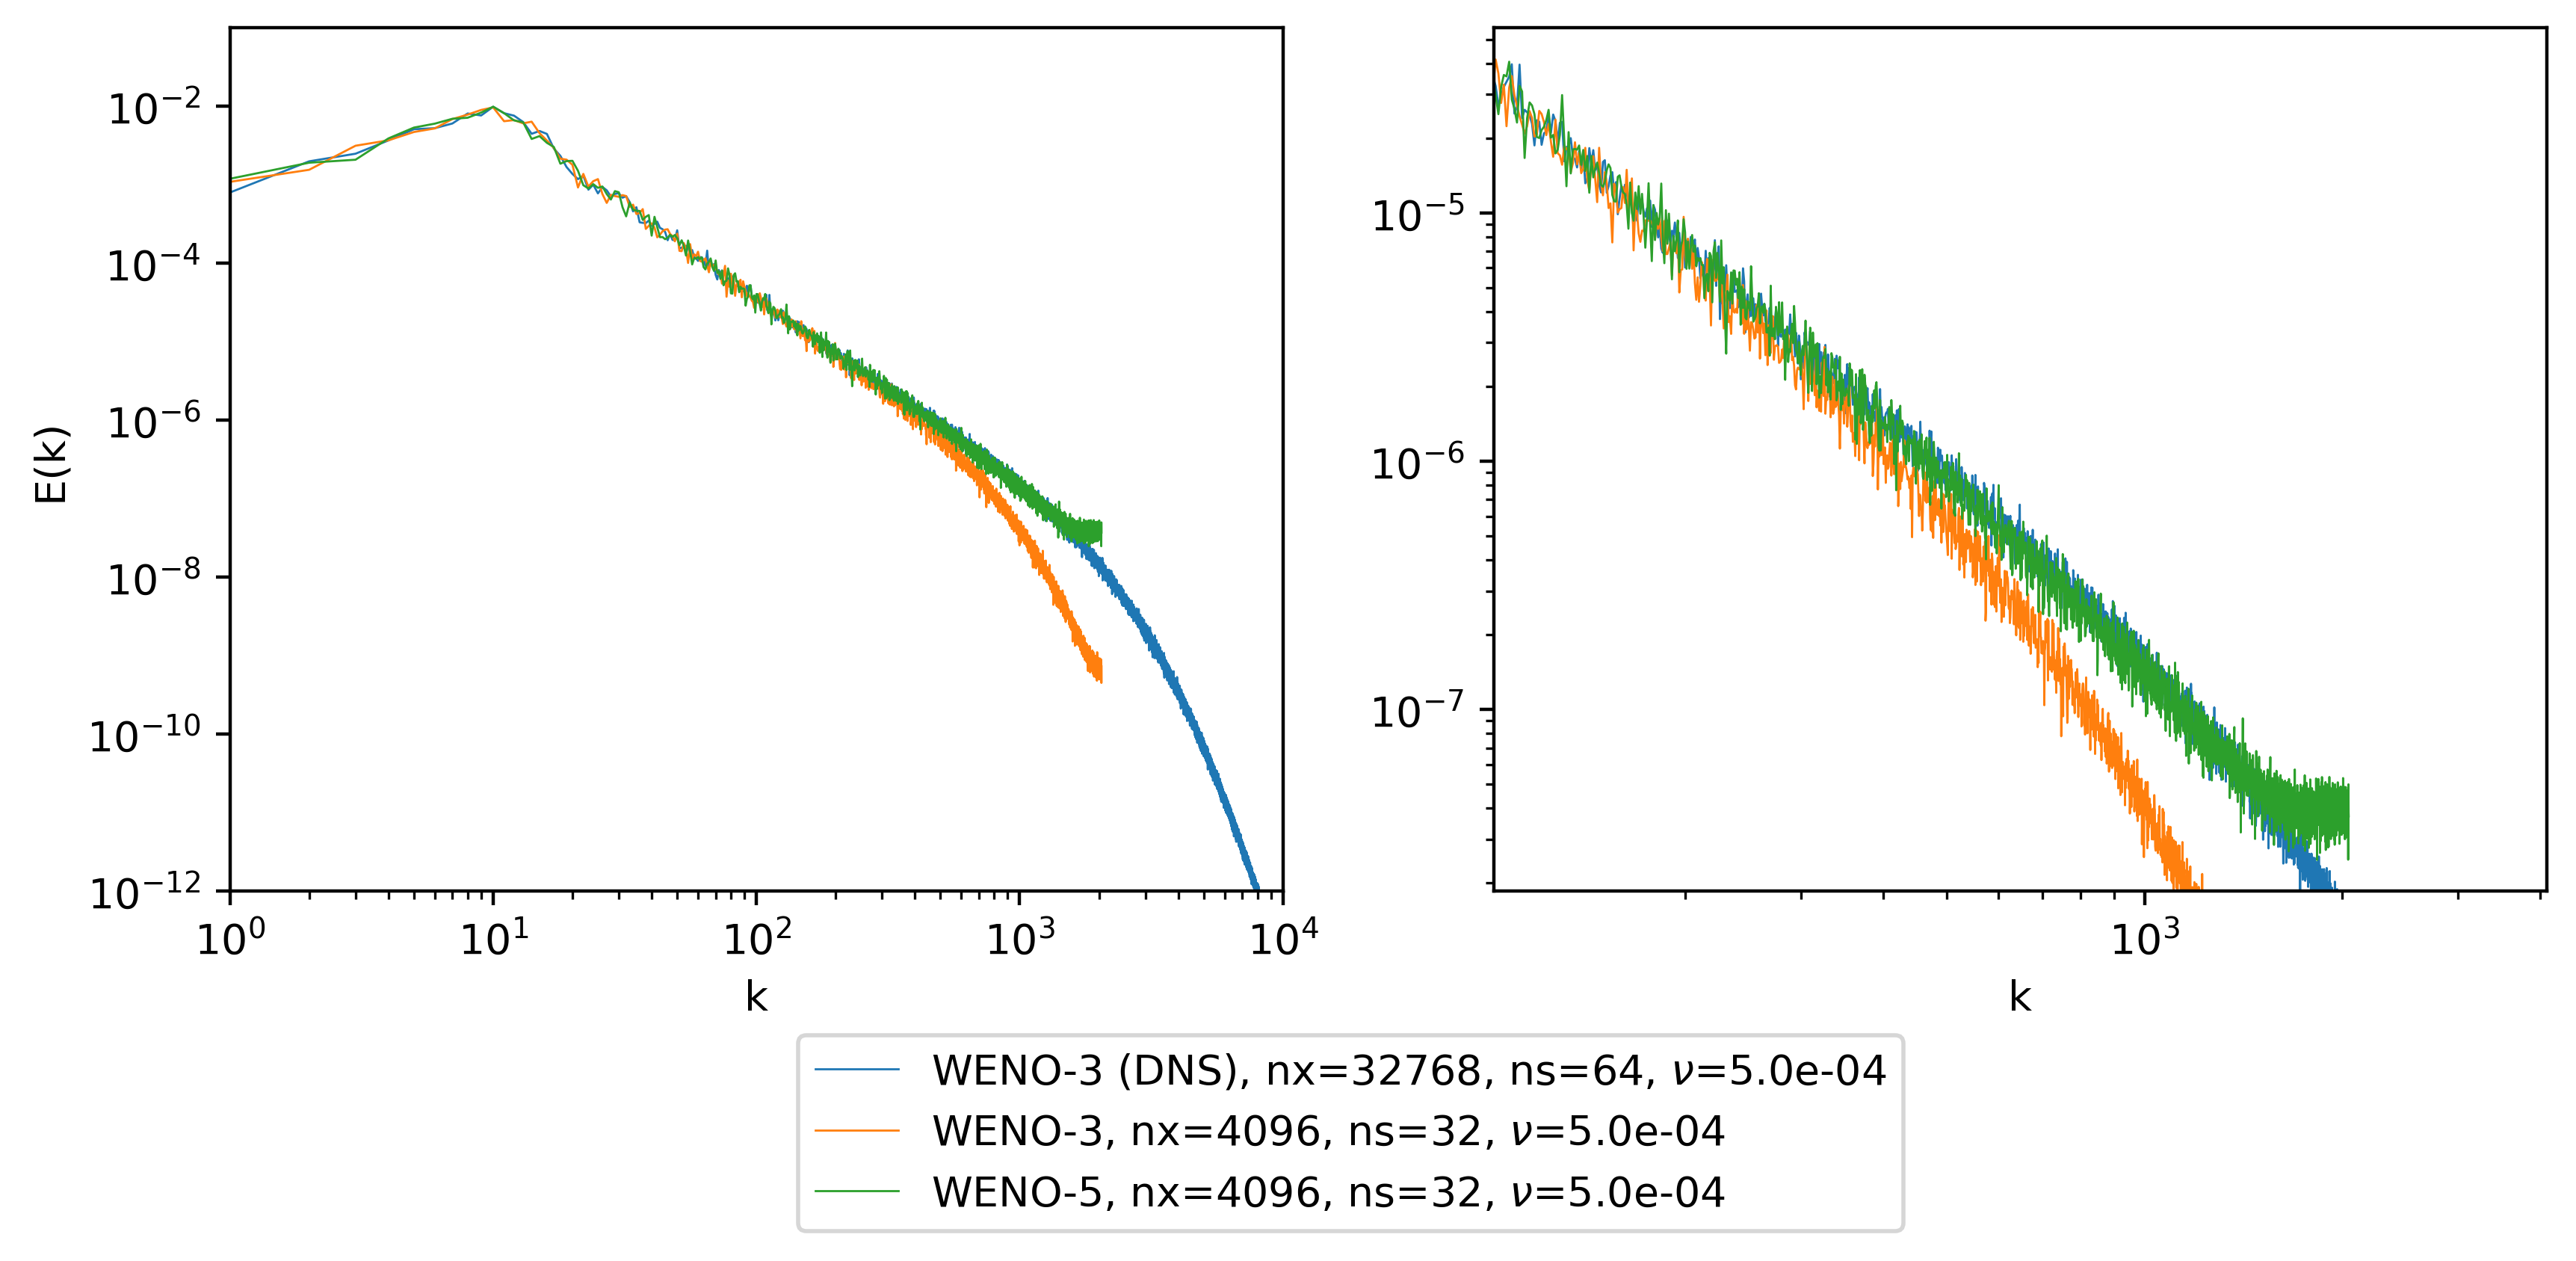
\includegraphics[width=0.7\textwidth]{figures/WENO_Order_Comparison_Ek_vs_k.png}
	\caption{WENO order comparison at $t=0.05s$}
	\label{fig:weno_order}
\end{figure}

\subsubsection{WENO-3 vs. WENO-5 for DNS} \label{sec:dns_type}o
With the decreased dissipation of the WENO-5 scheme, it might appear to be the
better choice for to use as the DNS result to compare other schemes against.
However, there are a couple of reasons it was not selected. First, the solution
for total kinetic energy over time was generally smoother for WENO-3 than
WENO-5 (see Figure \ref{fig:weno_order_diss_rate}). Second, as shown in Figure
\ref{fig:weno5_res}, WENO-5 exhibits dispersion errors near the edge of the
domain, making the solution less accurate at those points. This is also shown
in Figure \ref{fig:weno5_dns}, where WENO-5 is used as the "DNS" solution. The
consistently dispersive behavior of WENO-5 was a key factor in choosing WENO-3
as the DNS solution.

\begin{figure}[hbt!]
\centering

\begin{subfigure}[t]{0.49\textwidth}
	\centering
	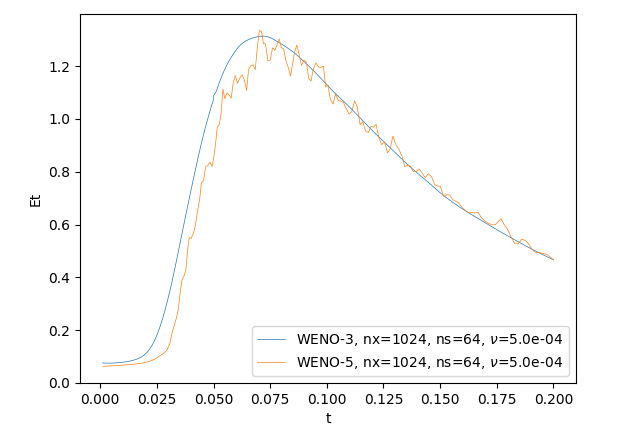
\includegraphics[width=0.99\textwidth]{figures/WENO_Order_1024_Et_vs_t.png}
	\caption{\label{fig:weno_order_diss_rate}}
\end{subfigure}
\begin{subfigure}[t]{0.49\textwidth}
	\centering
	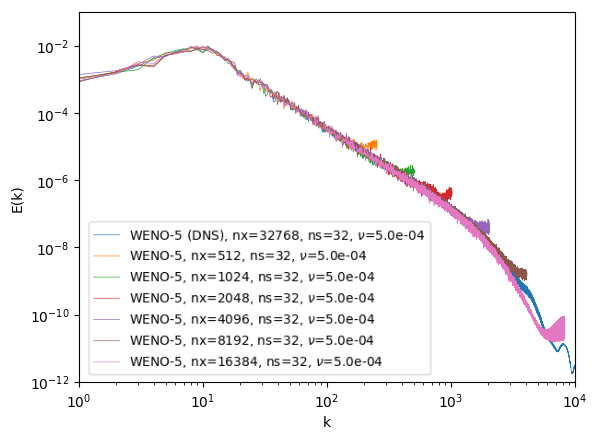
\includegraphics[width=0.99\textwidth]{figures/WENO5_DNS_Ek_vs_k.png}
	\caption{\label{fig:weno5_dns}}
\end{subfigure}

\caption{(a) WENO order comparison, kinetic energy dissipation rate at $t=0.05s$;
		 (b) WENO-5 resolution comparison with WENO-5 as DNS solution, $t=0.05s$}
\end{figure}

% \begin{figure}[hbt!]
% 	\centering
% 	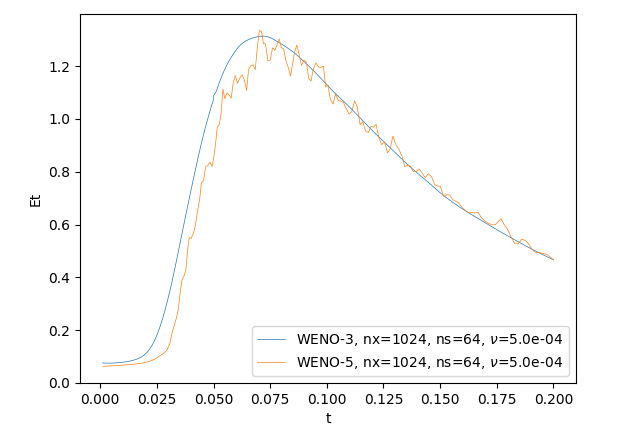
\includegraphics[width=0.6\textwidth]{figures/WENO_Order_1024_Et_vs_t.png}
% 	\caption{}
% 	\label{fig:weno_order_diss_rate}
% \end{figure}

% \begin{figure}[hbt!]
% 	\centering
% 	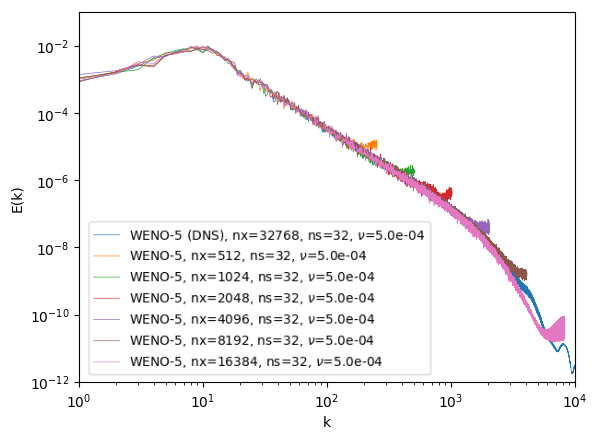
\includegraphics[width=0.6\textwidth]{figures/WENO5_DNS_Ek_vs_k.png}
% 	\caption{WENO-5 resolution comparison with WENO-5 as DNS solution, $t=0.05s$}
% 	\label{fig:weno5_dns}
% \end{figure}

\subsection{MUSCL vs. WENO Comparison} \label{sec:muscl_vs_weno}

Finally, the best MUSCL scheme was compared against WENO-3 and WENO-5 at the
same resolution and number of samples. The results, shown in Figure
\ref{fig:best_muscl_vs_weno}, show that WENO-5 follows the DNS result the
closest. However, because of its dispersive characteristics outlined in section
\ref{sec:dns_type}, it would seem that MUSCL-KT can be considered the least
dissipative scheme while remaining stable.

\begin{figure}[hbt!]
	\centering
	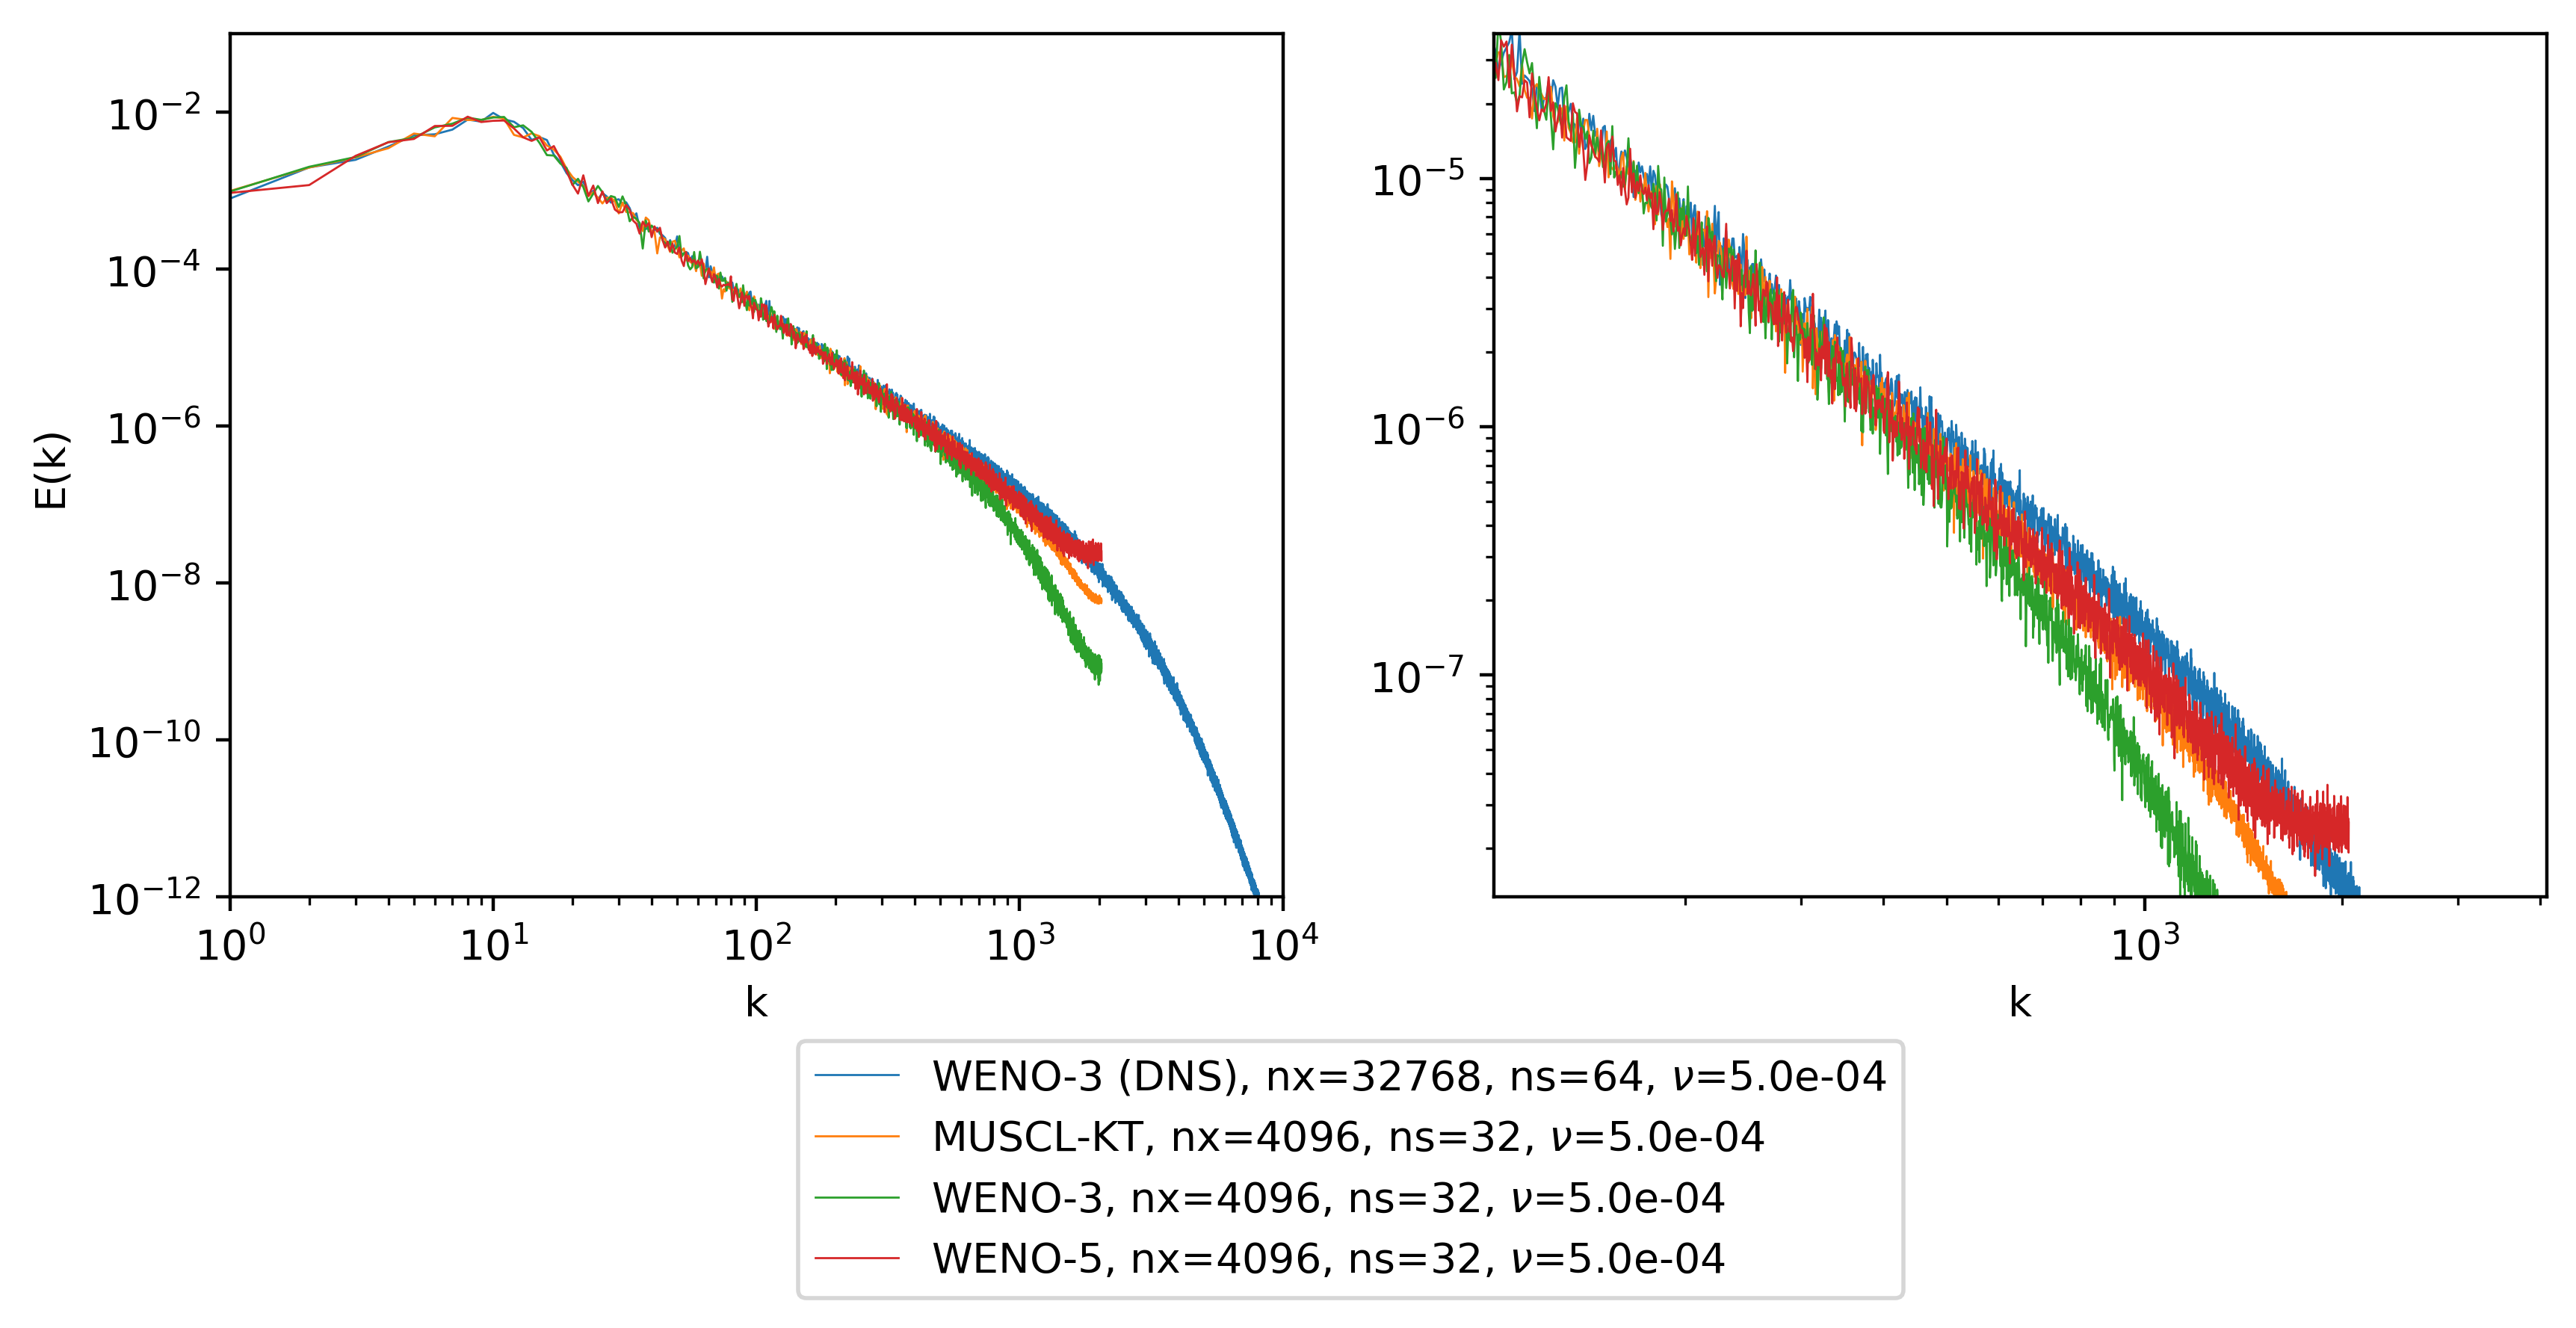
\includegraphics[width=0.7\textwidth]{figures/Best_MUSCL_vs_WENO_35_Ek_vs_k.png}
	\caption{Best MUSCL scheme vs WENO-3 and WENO-5, $t=0.05s$}
	\label{fig:best_muscl_vs_weno}
\end{figure}

\section{Conclusions}
In this study, various reconstruction schemes were investigated to compare
their dissipative and dispersive characteristics when solving the 1D viscous
Burgers turbulence problem. After analyzing many different MUSCL schemes,
limiters, and WENO schemes, it was determined that the MUSCL-KT scheme with no
limiter gave the least dissipative and dispersive solution for a given spatial
resolution. Further studies could compare these against flux-splitting schemes
and other reconstruction schemes. These could all be applied to a different set
of initial conditions, such as a shock, to see how the different schemes
perform for different scenarios.

\newpage

\bibliography{CP2}

\end{document}
